\documentclass[12pt]{report}
\usepackage[dvipdfmx]{graphicx}
\usepackage{url}
% \usepackage[hidelinks]{hyperref}
\usepackage{jaist-e-doctor}

\title{% Write title of your thesis 
Dimensional Speech Emotion Recognition by Fusing Acoustic and Linguistic Information}
\author{Bagus Tris Atmaja}
\school{Graduate School of Advanced Science and Technology}
\adviser{Professor Masato Akagi}
\date{Information Science \\ \today}

\begin{document}
\maketitle

\pagenumbering{roman}  % Show page number in ROMAN 
\setcounter{page}{1}

\strut
\vspace{20pt}

\begin{center}
{\LARGE\bf Abstract}
\end{center}
\vspace{20pt}
\addcontentsline{toc}{chapter}{Abstract}

This paper investigates the error 
correcting capabilities of concatenated codes 
employing maximum distance separable (MDS) codes as outer codes and
time-varying randomly selected constant composition inner codes,
used on discrete memoryless channels with modified maximum mutual 
information decoding. It is proved that such code
can achieve Gallager's random coding error exponent
for all rates, while both encoding and decoding of the codes do not
depend on the channel. 

\renewcommand{\nomname}{ACKNOWLEDGMENTS}
\markboth{\nomname}{\nomname}

\strut
\vspace{20pt}

\begin{center}
{\LARGE\bf Acknowledgments}
\addcontentsline{toc}{chapter}{Acknowledgments}
\end{center}
\vspace{20pt}

% thank to prof akagi
The author wishes to express his sincere gratitude to his principal supervisor,
Professor Masato Akagi of Japan Advanced Institute of Science and Technology,
for his constant encouragement and kind guidance during this dissertation work.
Prof. Akagi not only guides the author to the research direction but also
pushes the timeline of the author's research to stay on track. Prof. Akagi is a
role model of supervisor for granting ``license" for prospective researcher, a
Ph.D. candidate. 

% thank to prof Unoki
The author also wishes to express his thanks to Professor Unoki, the
co-supervisor of this dissertation. Without his critical questions, some parts
of this doctoral study will not exist. The author owes the idea of multitask
learning and silent pause feature calculations to Prof. Unoki.

% thank to prof Shirai
The author is grateful to Professor Kiyoaki Shirai for his helpful suggestions
and discussions during minor research. With the acoustic information science
background, the author has no sufficient knowledge of linguistic information
processing until conducting minor research in his lab. His patience and
kindness accelerate the author's understanding of the use of linguistic
information for dimensional speech emotion recognition.

% thank to AIS member
The kind, friendly, and warm environment at Acoustic Information Science-Lab
(Akagi and Unoki Lab) was the ideal place for conducting research and study.
Surrounded by forests and natural landscapes, there is no better place for 
Ph.D. study except in JAIST. The author would like to thank all AIS members for
their kindness support during his Ph.D. study.

% thank to MEXT
Funding is one of the crucial factors when conducting research. The author
would like to thank the Ministry of Education, Culture, Sports, Science, and
Technology (MEXT) of Japan for granting a scholarship for his studies.

Finally, the author would like to thank his family and friends. This
dissertation is dedicated to them. 

% Finally, time is short, writing is hard, and thesis is
% long. This thesis is endurance test for facing the short, the hard, and the
% long.


\tableofcontents
\listoffigures
\listoftables
\newpage
\pagenumbering{arabic}
\setcounter{page}{1}

\newtheorem{theo}{Theorem}
\newtheorem{lemma}{Lemma}
\newtheorem{col}{Corollary}
\newtheorem{defini}{Definition}
\newtheorem{pro}{Property}
\def\bm#1{\mbox{\boldmath{$#1$}}} \def\eqtri{\stackrel{\triangle}{=}}
\def\c#1{#1^{\dagger}} \newcommand{\gf}{\mbox{$GF(q)$}}
\newcommand{\av}[1]{\mbox{E${\displaystyle\left[ #1 \right]}$}} \def\r{\bm{r}}
\def\s{\bm{s}} \def\w{\bm{w}} \def\x{\bm{x}} \def\y{\bm{y}} \def\a{\bm{a}}
\def\u{\bm{u}} \def\cX{{\cal X}} \def\cY{{\cal Y}} \def\cP{{\cal P}}
\def\cV{{\cal V}} \newcommand{\g}{\mbox{$\Gamma$}}
\def\qed{\strut\hfill(Q.E.D.)} \def\eot{\strut\hfill$\Box$}
\def\osum{\bigcirc\hspace{-1.2em}\sum} \newcommand{\vt}[1]{\mbox{\boldmath
$#1$}}

\chapter{Introduction}
This chapter introduces the necessary background to conduct research on
dimensional speech emotion recognition. The aims, problems, concept,
contributions, and structure of the dissertation are also briefly presented as
guide in navigating the following chapters.

\section{Background}
Emotion can be regarded as the major difference between humans and computers.
At the beginning of human-computer interaction (HCI) development, no computer
would understand human emotion. Nowadays, there have been attempted to
recognize human emotion automatically by computers. If a computer could
correctly recognize emotion, HCI would be benefited greatly. For example, 
vehicle could detect driver's mood (long time emotion) to ensure safety. In
other applications, the satisfaction and performance of user and operator
through call center applications can be measured using speech emotion
recognition technologies.

Speech emotion recognition (SER) is an emerging technology that is resulted
from science in multi-discipline area, including psychology, physiology,
acoustics, and affective computing. The psychology of emotion focuses on how a
human reacts to certain stimuli and how these stimuli affect both mentally and
physically of humans. The physiology of emotion is related to arousal of the
nervous system with various states and strengths of arousal relating to
particular emotions. The acoustic of emotion studies on what acoustic features
relate to human emotion. The latter affective computing, according to Picard
\cite{Picard}, is termed as ``computing that relates to, arises from, or
influences emotion."

% add definition and rationale for linguistic information
Aside from those disciplines, language also has an impact on the expression of
emotion. Humans communicate emotion through speech and language
\cite{Kotz2011}. Furthermore,  language is argued to shape perceived emotion
intrinsically \cite{Lindquist2006}. Thus, utilizing linguistic information in
automatic SER may be useful to make computer accurately recognize human
emotions. 

% add definition of information science
Information science is a study of using information processing to find a
solution to an important social problem. In information science, a hierarchy of
data-information-knowledge (DIK) is known to model the flow of data. This model
can be used to model emotion recognition. The input to the data is signal,
which is an acoustic signal in SER. The data is the speech dataset. The
information is the features (acoustic and linguistic). The knowledge is the
degree of dimensional emotion. This concept, which will be explained in more
detail in Chapter 3, correlates information science with SER or models SER from
an information science perspective. 

% acoustic information science
Acoustic information science is the study of information science for acoustic
phenomena -- phenomena relate to sound. Speech is part of acoustic information
science; thus, the study of speech involves concepts used in acoustic
information science (e.g., acoustic signal processing). SER, although
multidisciplinary research, involves two main fields, the acoustics of speech
and the psychology of emotion. For automatic SER by computers, the
understanding of speech acoustics and computer algorithms will provide a
necessary foundation for building a better SER system.

% Back to SER, why studying SER with multidisciplinary research
This experimental study explores the necessity of fusing acoustic and
linguistic information for dimensional emotion recognition. The study views SER
from an acoustic information science point of view. Speech contains both
linguistic (verbal) and acoustic (non-verbal) information. While the
conventional SER method only uses acoustic information, fusing both acoustic
and linguistic information exists in human-human communication and is feasible
for human-computer interaction.

\section{Research aims and problems}
Speech is the primary modality for communication (known as speech
communication) including communicating human emotions. Even if other modalities
may influence on how human communicate emotions (e.g., facial expressions,
gesture, posture, body's motion/movement, and other physiological signals), in
special cases, like in telephone calls or voice assistant applications, 
speech is the only modality to determine a speaker's emotion.

In certain cases, using acoustic information only (e.g., prosody or intonation)
to perceive human emotions may be not enough. For instance, happy and angry
voices may have similarities in high intonation, sad and fear may have
similarities in low intonations. In this case, knowing the semantic of the
spoken words will increase the probability to recognize the perceived emotion
from speech. If the words have positive meanings and are uttered with high
intonations, then the chance that the speaker was happy is higher than angry.
This bimodal information fusion of acoustic and linguistic could be implemented
in computer algorithms to improve the performance of SER.

Thus, combining acoustic and linguistic information is relevant for improving
SER performance by computers. There is no need to add additional modalities
since linguistic information can be derived from speech. Modern automatic
speech recognition (ASR) can produce text in almost real-time processing. The
transcribed spoken text can be used to extract linguistic information. Both
acoustic and linguistic information can be fused in such frameworks to evaluate
the effectiveness of information fusion over unimodal information.

The main goal of this research is to investigate the necessity of fusing
acoustic information with linguistic information for dimensional SER. To
achieve this main goal, the following three sub-goals were addressed: 
\begin{enumerate}
\item maximizing the potency of SER from acoustic information only by
investigating the region of analysis and silence region for feature extraction,
\item studying the fusion of acoustic and linguistic information at the feature
level (early fusion) and its effect, particularly for valence prediction
improvement, and 
\item studying the fusion of acoustic and linguistic information at the decision
level (late fusion) and comparing the results with the previous approach.  
\end{enumerate}

There are five problems to be solved by these goals. The first problem is the
region of analysis for acoustic feature extraction. The second problem is the
effect of silent pause region in dimensional SER. The third problem is the low
performance of valence prediction. The fourth problem is the necessity to fuse
acoustic information and linguistic information for dimensional SER. The fifth
problem is to find the effective fusion framework for combining acoustic and
linguistic information. Figure \ref{fig:aims_issues} shows the connections
between research aims and research problems. The details of these aims (which
is transformed into research strategies) and problems (issues) are discussed
further in Chapter 3. 

\begin{figure}[htbp]
    \centering
    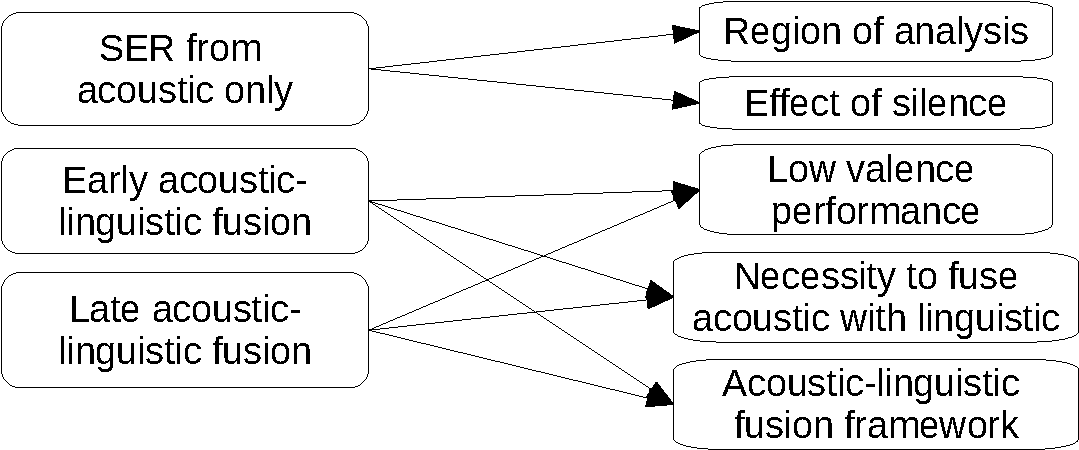
\includegraphics[width=0.7\textwidth]{../fig/aims_issues-crop.pdf}
    \caption{Connection between research aims (left) and research problems (right)}
    \label{fig:aims_issues}
\end{figure}

\section{Research concept}
% explains research concept: speech is not only about how but what
Speech delivers a message that goes beyond words. In this understanding, word
meaning is not enough to convey a message; acoustic information is needed.
Acoustic information alone is also not enough to deliver a message. It is not
only how it is said (acoustic), but also what is said (linguistic).
This concept is the foundation of this research, shown in Figure
\ref{fig:concept}. 

\begin{figure}[htbp]
    \centering
    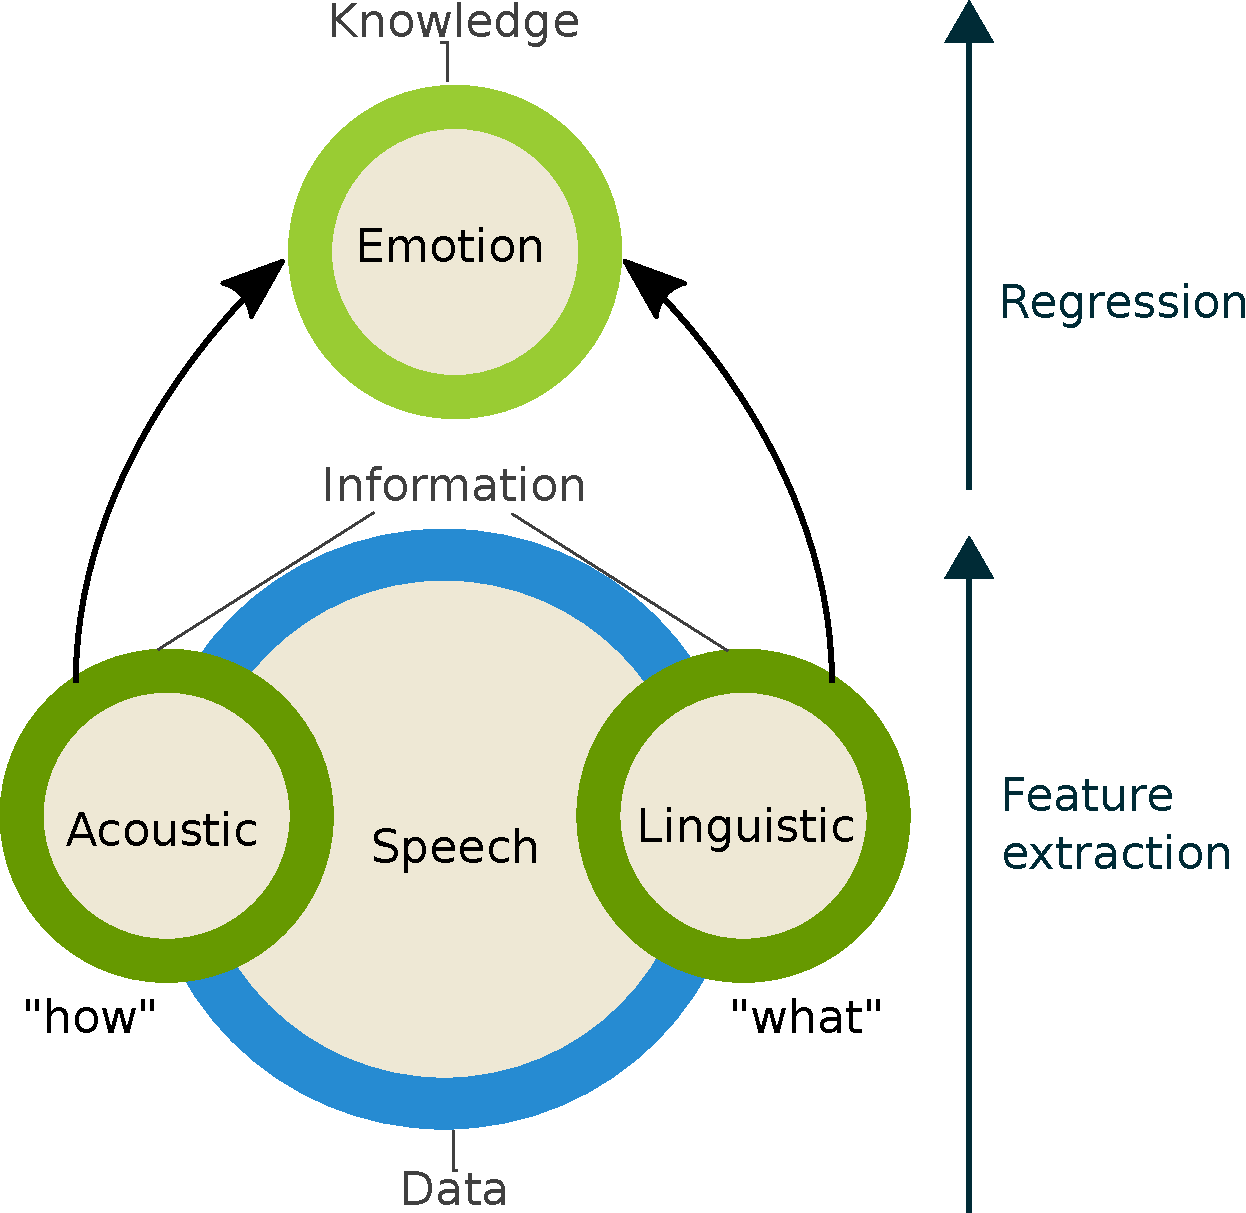
\includegraphics[width=0.6\textwidth]{../fig/concept-rev.pdf}
    \caption{Research concept of dimensional speech emotion recognition by fusing acoustic and linguistic information}
    \label{fig:concept}
\end{figure}

This research concept differs from the previous studies (e.g., \cite{Li2019b,
Vayrynen2014}). In these studies, the belief for speech is about how it is said
rather than what is said. This study combines both ``how'' and ``what''
information. Acoustic features contain information on how it is being said.
Linguistic features contain information on what is being said. Fusing both
pieces of information, which are extracted from a speech, will improve the
clarity of the message, including the expressed emotion. The perception of
emotion will also improve by fusing this bimodal information. Figure
\ref{fig:concept} shows the concept of automatic recognition of dimensional SER
by fusing both pieces of information. This process is also in line with the
previous DIK concept in information science.

The process of recognizing emotion from speech consists of two main steps.
First is extracting information from speech data; second is extracting degree
of dimensional emotions as knowledge from acoustic and linguistic information.
Features extraction extracts two pieces of information from speech --- acoustic
and linguistic. Since dimensional SER is a regression task, a regression
process will map extracted features to the ground truth labels. This process is
commonly performed within machine learning or deep learning. The acoustic and
linguistic information are fused in this step, which can be implemented in
various ways.

\section{Contributions}
The contributions of this dissertation can be traced to the published papers.
These contributions can be divided into three areas, as follows.
\begin{enumerate}
\item Acoustic feature extraction \\
In \cite{Atmaja2019} the author evaluated categorical speech emotion
recognition from silence-removed speech region. The result suggests that
extracting acoustic features from the silence-removed region is better than
from the whole speech region. In \cite{Atmaja2020f}, the author utilized
silence as an additional feature to statistical functions. The results achieved
a better score than baseline raw speech. The author confirms and generalizes
the effectiveness of mean and standard deviations of low-level acoustic
features for SER \cite{Atmaja2020f, Atmaja2020d}. In \cite{Atmaja2020h}, the
author showed that acoustic feature aggregation leads to better performances
than output aggregation. These contributions are explained in Chapter 4. In
\cite{Atmaja2020j}, the author found that the acoustic features that perform
better in SER will also perform better in song emotion recognition.

\item Information fusion \\
In \cite{Atmaja2019b, Atmaja2020d, Atmaja2020h}, the author proposed emotion
recognition by fusing acoustic and linguistic information at feature level. The
results significantly improved unimodal dimensional emotion recognition from
either acoustic or linguistic information. Furthermore, the author discussed the
improvement of valence prediction in \cite{Atmaja2020e}. While this
contribution is discussed in Chapter 5, the improved version of the proposed
method, the late fusion method, is explained in Chapter 6. The evaluated fusion
methods are expanded not only for acoustic and linguistic fusion but also for
acoustic and visual information fusion \cite{Atmaja2020, Elbarougy2020}. 

\item Classification methods \\ 
Modern classification methods utilized deep learning models. However, the
conventional method, such as support vector machine (SVM) and multi-layer
perceptron (MLP), are still used in many fields. The author showed that
traditional MLP with deeper layers and proper configurations performed better
than modern deep learning architecture \cite{Atmaja2020k}. For the SER task
with deep learning, the author confirmed the need for bigger data size to be fed
to deep learning models \cite{Atmaja2019c}. The choice of the loss function is
a matter in machine/deep learning. The author proposed correlation-based loss
function to improve the performance of dimensional SER \cite{Atmaja2020,
Atmaja2020d,Atmaja2020b}. The author also evaluated multitask learning (MTL)
for predicting valence, arousal, and dominance degrees simultaneously based on
this loss function \cite{Atmaja2020d, Atmaja2020i}.  Furthermore, the author
found that recurrent-based neural networks (RNN) are effective for the SER task
\cite{Atmaja2019a}. More improvements were obtained when this RNN model is
combined with the attention model \cite{Atmaja2019}.
\end{enumerate}


\section{Dissertation structure}
This dissertation is organized in eight chapters. The rest of these chapters is
organized as follows.
% a visualisation of this structure is
% illustrated in Figure \ref{fig:dissertation_org}.
\begin{itemize}
\item \textbf{Chapter 2} presents a literature study on speech emotion
recognition from bimodal acoustic and linguistic information fusion. An
introduction that motivates the previous research by fusing acoustic and
linguistic information is presented. This chapter reviews the models, features,
classifiers, and fusion methods for the SER task.
\item \textbf{Chapter 3} describes the research methodology --- justification
for using particular research methods. This chapter consists of the motivation
of researching SER, research issues, research philosophy, research strategies,
datasets, and a description of an evaluation metric. 
\item \textbf{Chapter 4} describes SER by using acoustic features. This chapter
investigates the region of analysis, the effect of silent pause features, and
the aggregation methods for acoustic-based SER.
\item \textbf{Chapter 5} describes the fusion of acoustic and linguistic
information at the feature level. This chapter evaluates the concatenation of
features and networks for bimodal emotion recognition from acoustic and
linguistic information. A SER evaluation from automatic transcription is also
provided in addition to manual transcription.
\item \textbf{Chapter 6} describes the fusion of acoustic and linguistic
information at the decision level. This chapter evaluates the late-fusion
approach by combining both information on two steps processing, including some
related issues: speaker-dependent vs. speaker-independent scenarios and effect
of lexical-controlled lexicons.
\item \textbf{Chapter 7} compares the results within this study and with other
studies. 
\item \textbf{Chapter 8} presents the overall conclusions of the dissertation.
Some possible future research directions are proposed from the current research
findings.
\end{itemize}

This dissertation's organization is summarized in Figure
\ref{fig:dissertation_org}. 

\begin{figure}[htbp]
    \centering
    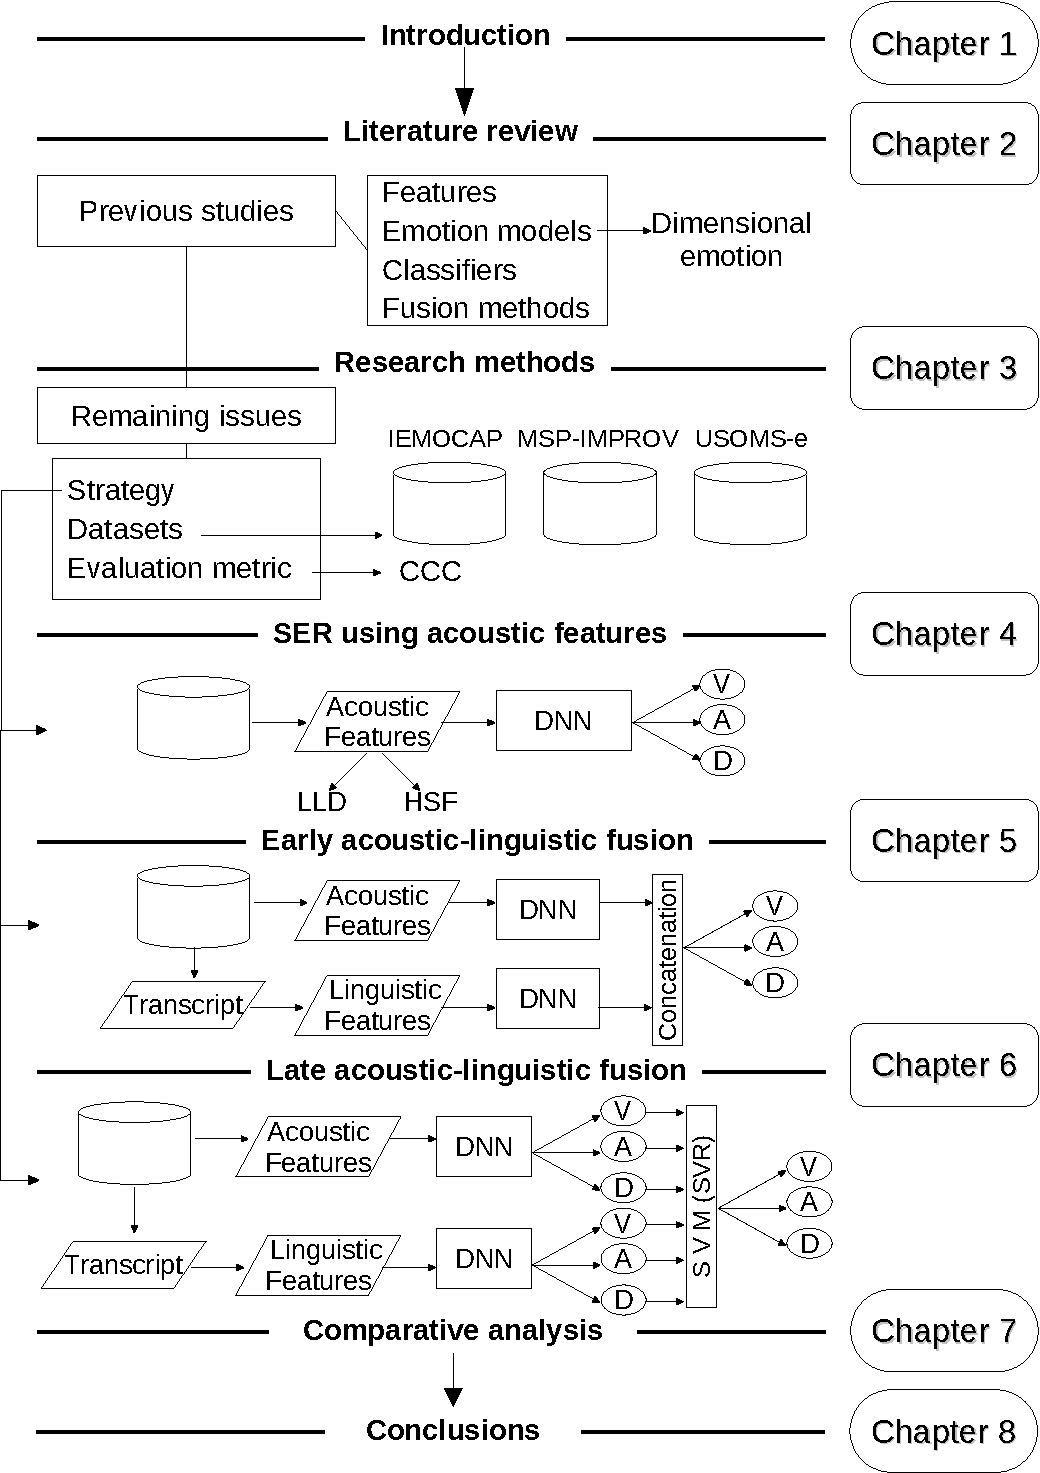
\includegraphics[width=.95\textwidth]{../fig/dissertation_org-crop.pdf}
    \caption{Organization of the dissertation}
    \label{fig:dissertation_org}
\end{figure}

% \newpage
% \thispagestyle{empty}
% \mbox{}

\chapter{Literature Review}
% this chapter will be submitted to ATSIP This chapter reviews speech emotion
% recognition from bimodal information: acoustics and linguistics.  This
% section aims to outline the progress of research on speech emotion
% recognition recently. This outline includes emotion models, datasets,
% features and classifiers.  always ask why?!

This chapter reviews research on speech emotion recognition from two
modalities, acoustic and linguistic information. Four main components of speech
emotion recognition from multimodal fusion are described, including emotion
models; features; classifiers; and fusion methods. Each section after
Introduction describes each of these components with their advancements and
current limitations; the last section summarizes this chapter.

\section{Introduction}
% history of SER
Speech emotion recognition (SER) is a part of affective computing that relates
to, arises from, or influences emotions \cite{Picard} within speech. SER is an
attempt to make the computer to be able to recognize expressed emotion in a
given utterance. The earliest reported research on SER, perhaps, was the work
of Dellaert et al. \cite{Dellaert}. The study explores prosodic features with
several statistical pattern recognition techniques to classify the emotional
content of utterances. Under a limited number of data (1000 utterances), the
system achieved a comparable performance close to humans. 

% Why speech -- another milestone
Utilizing speech to identify humans' emotions rooted from the correlation
between voice and emotion. There is strong evidences that humans can recognize
other's emotions from their voices. In addition, given that speech is less
private than image and video, using speech to recognize emotion benefits future
implementation. Another milestone conducted by Petrushin \cite{Petrushin1998}
prove a pilot study to implement SER for call center application. This
laboratory-scale study, at that time, showed a potential application for SER
technologies.  Nowadays, this SER technology is ly available in the
commercial market, while its research is still ongoing. 

% SER dataset development (2000-2010)
The potential application of speech-based emotion recognition triggers the need
for such datasets. During 2000s, several datasets for emotion recognition
have been published, including the availability of speech data in the datasets.
Among many datasets, the following are commonly used in SER research: EmoDB
\cite{Burkhardt2005}, IEMOCAP \cite{Busso2008}, MSP-IMPROV \cite{busso2016msp},
and RAVDESS \cite{Livingstone2018}. The availability of these datasets
accelerates research on the SER area.

% SER in the modern era (2010-)
The progressive research on SER led to practical implementation in the
commercial industry. Nowadays, SER has been implemented in various
applications, both web/cloud-based applications or standalone applications.
Although it is useful to analyze the subject's affective state, these emerging
affective recognizer technologies have been criticized by others. Researchers
in psychology argued that due to individuals' high variability, the emotional
categories do not have an essence. The correlation between
particular facial expression and the corresponding basic emotion was not
strongly supported \cite{Barrett2019}. 

% Why fusing acoustic and linguistic: multimodal --> bimodal
Among many other issues, multimodal information fusion is a challenging task in
pattern recognition. Recent studies (e.g., \cite{Poria2017,Atmaja2020d,
Atmaja2020, Atmaja2019b}) confirm that multimodal classifiers outperform
unimodal classifiers. In SER itself, one of the main issues in searching for a
more predictive feature is whether it suffices to explore acoustic features
only, or it is necessary to combine acoustic features with other modalities
\cite{ElAyadi2011}. For speech, both acoustic and linguistic features can be
extracted. Thus, two pieces of information can be fused to evaluate the
effectiveness of information fusion from a single speech modality.

% why add text
The use of linguistic information for SER is also reasonable from an affective
computing point of view. In task-processing related tasks, linguistic
information is extracted from the text for sentiment analysis. This textual
information was also used to detect emotion in text
\cite{Alm2005,Mulcrone2012,Calvo2013}. In these works, textual information
showed encouraging results on both categorical and dimensional emotion
recognition from text. Fusing acoustic and linguistic information may improve
the performance of SER more significantly than other strategies.

% Shows bimodal results
Indeed, bimodal emotion recognition by fusing acoustic and linguistic
information shows significant performance improvement. References
\cite{Schuller2004,Schullera,Eyben2010,Ye2014,Tian2019} show the usefulness of
fusing acoustic and linguistic in different strategies to improve SER
performance. Different acoustic and linguistic features were fused using
different classifiers. Different fusing strategies were evaluated to
investigate the effectiveness of the fusion method.

% purpose of the chapter
This chapter aims to review current studies of bimodal emotion recognition by
utilizing acoustic and linguistic information. The scope of this study includes
the emotion models, features, classifiers, and fusion methods used in bimodal
SER. In the end of this chapter is a summary concluding this literature review.


% Although there are hundreds of research papers on speech emotion recognition,
% only 50s papers focused on bimodal emotion recognition by accommodating
% acoustic and linguistic information.

\section{Emotion models}
Before beginning to research emotion recognition, it is important to choose
which emotion model to adopt. According to \cite{Grandjean2008}, there are at
least three views to model humans' emotions: categorical emotion, dimensional
emotion, and componential appraisal emotion. However, all SER research employed
either first, second, or combination of both views as target emotion.  No
research was found on using speech data to obtain appraisal emotion. Thus, the
following description describes major models in active affective computing
research. 

\subsection{Categorical emotion}
Categorical emotion, also known as basic emotions, is the discrete emotion that
is independent of each other in its manifestations. Although the original idea
is to organize affective state into their emotion families (rather than
discrete emotion); however, most researchers agree that there are six basic
emotions: anger, fear, enjoyment, sadness, disgust, and surprise. The first
five emotions are backed by robust and consistent evidence, while the evidence
for the surprise is not as firm \cite{Ekman1992}. Nevertheless, these six basic
emotions have been a standard in categorical emotions.

Before Ekman coined the terms of basic emotions, Plutchik
\cite{plutchik1980emotion} have defined basic eights bipolar emotions: joy
(reproduction), sorrow/sadness (deprivation), acceptance/trust (incorporation),
disgust (rejection), surprise (orientation), anticipation (exploration), anger
(destruction), fear (protection). These eight emotions can be illustrated as a
wheel of emotion, as shown in Figure \ref{fig:plutchik_model}. Each emotion can
mix with other emotion to make up another emotion, as mixing colors. 

\begin{figure}[htbp]
    \centering
    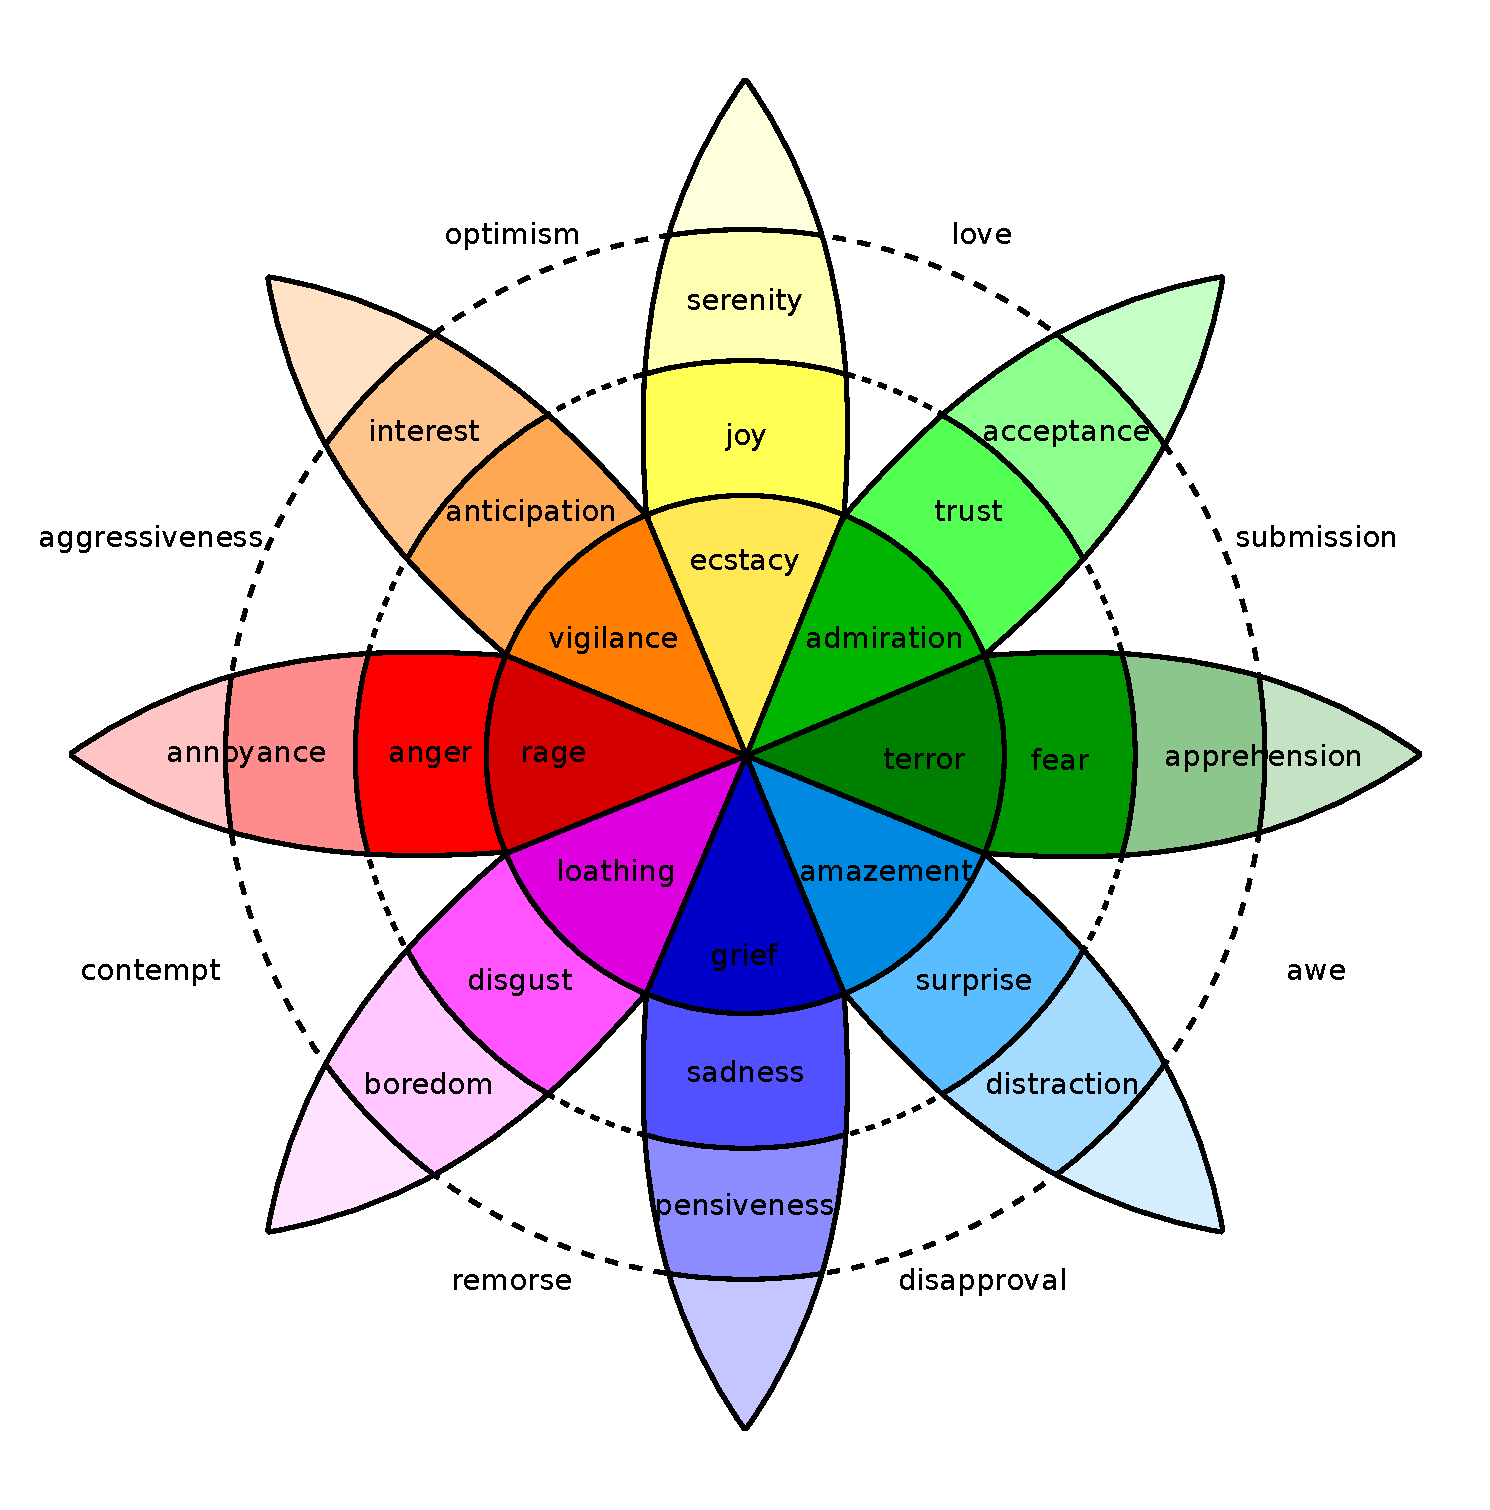
\includegraphics[width=4in]{../fig/plutchik_model.pdf}
    \caption{Plutchik wheel of emotions}
    \label{fig:plutchik_model}
\end{figure}

Instead of six, recent research suggests that four latent expressive patterns
were commonly observed in facial expressions \cite{Jack2016}. However, instead
of mentioning the name of basic emotions, the research utilized the term basic
"action unit pattern" (AU Pattern), from one to four. Although backed by
scientific evidence, this finding did not have any practical implementation
yet.

Ekman revised the characteristics which distinguish basic emotion from 9
criteria \cite{Ekman1992} to 11 criteria \cite{Ekman2005}. The new criteria
resulted in 15 emotions: amusement, anger, contempt, contentment, disgust,
embarrassment, excitement, fear, guilt, pride in achievement, relief,
sadness/distress, satisfaction, sensory pleasure, and shame. Du et al. 
\cite{Du2014} shows 21 categories of facial expressions by a facial action
coding system analysis. Furthermore, Cowen and Keltner \cite{Cowen2017} found
27 emotional experiences from facial expression by across self-report methods.
The growth of the number of categorical emotions, based on facial expression
measurement, confirms the high variability of humans expressed emotions. Darwin
argued that the biological category, including the emotion category, does not
have an essence; it is hard to map one-to-one facial expressions to emotional
states.

% closing statement for journal paper there is missing link from pyschological
% research to AI research. In psychologyical research unfound correlation
% between particular facial expression and related emotion. In contrast, AI
% research found that facial information is the richest modality to extract
% emotion from humans.  Most research on dividing emotion into categories were
% based on facial expression. Given inconsistency results, it is interesting to
% explore the possibility to find "fingerprint" of emotion in speech. In other
% words, what is the most important acoustic feature related to emotion?

% Most research conducted in SER were done from speech processing (engineering)
% point of view. It will be interesting to see results of psychoacoustics
% result of emotional speech (speech science). The investigation of particular
% emotion (e.g., anger) with its acoustic characteristics is a merit study.

\subsection{Dimensional emotion}
Instead of dividing emotion into several categories, a dimensional emotion
views emotion as continuous values/degrees of attributes in valence-arousal
space (VA) or valence-arousal-dominance (VAD) space. Valence is the degree of
positive or negative emotion, arousal refers to the level of activation from
sleepiness (low) to awakeness (high), and dominance is the degree of control
over the emotion \cite{Gunes2010}. In this theory, an emotion or affective
state is not independent of one to another. Rather, they are related one to
another in a systemic manner (in VA or VAD space). Russel argued that the
previous categorical emotion could be mapped within VA spaces. An illustration
of VA space with several emotion categories is shown in Figure
\ref{fig:va_space}.  


\begin{figure}[htbp]
    \centering
    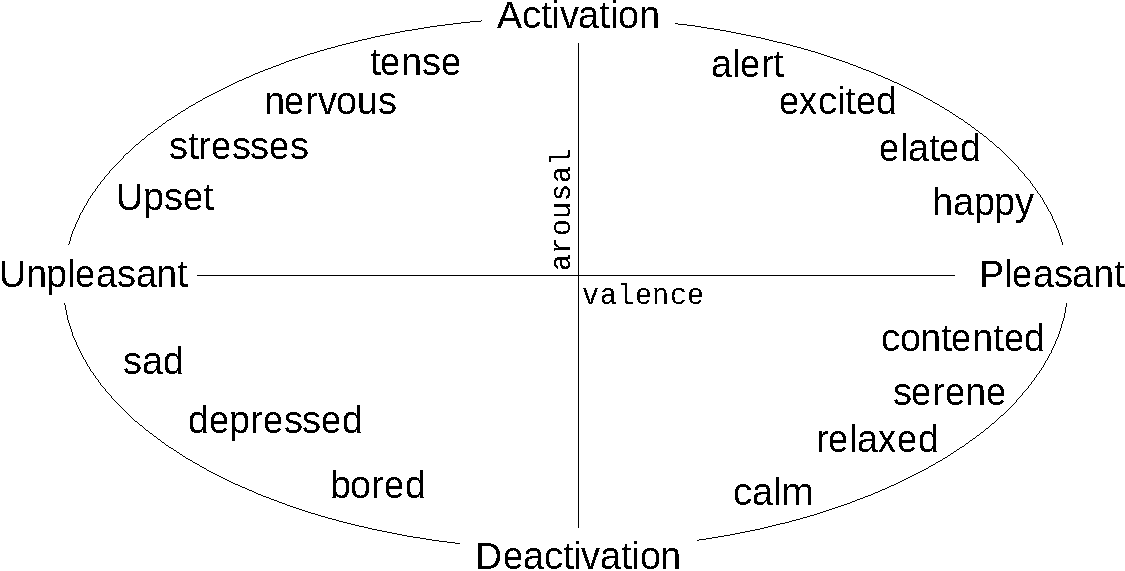
\includegraphics[width=.8\textwidth]{../fig/circumplex-crop.pdf}
\caption{Graphical representation of circumplex model (VA
space)\cite{Posner2005}; vertical axis: arousal; horizontal axis: valence}
    \label{fig:va_space}
\end{figure}

The search for higher dimensions for dimensional emotion is a worthwhile study.
Russel argued that all emotion categories could be mapped in 2D valence-arousal
space \cite{Russell1980a}. However, Fontaine et al. have found that the world
of dimensional emotion is not two or three dimensions, but four dimensions
\cite{Fontaine2017}. The fourth dimension is the unpredictability. In order of
importance, the order of dimensional emotions is valence, dominance, arousal,
and predictability. Fortunately, the similar fourth dimension is proposed in an
emotion recognition challenge \cite{Schuller2012}. In this challenge,
four-dimensional emotions were arousal, expectancy, power/dominance, and
valence. Expectancy, which represents the predictiveness of the subject's
feeling, is very similar to predictability/unpredictability in the previous
report.

The third emotion model, hybrid model or appraisal model, can be viewed as an
extension of the dimensional model. In this model, emotion categories are
spanned between bipolar dimensions. For instance, ``impatience" is located in
the upper part of the arousal axis (see \cite{Scherer2005}). This study of
appraisal-based emotion theory leads to the development of the Geneva emotion
wheel (GEW) rating study. This hybrid model has two similarities with the
previous 4D dimensional emotion model. First, the hybrid model also uses four
attributes (i.e., dimensions): valence, dominance/power, arousal, and
conducive/obstructive (instead of predictiveness). Second, in version 2.0 of
GEW, two axes used to draw emotion terms are valence and dominance/power, which
are the two most important emotional attributes according to
\cite{Fontaine2017}. Nevertheless, the use of the hybrid model in SER is not
familiar in the SER research community, perhaps due to these labels'
availability in the dataset.

\section{Features}
The input features to the SER system is the most important issue for developing
bimodal information SER. If the input is not informative for predicting emotion
or does not correlate to the predicted emotion, the prediction results will
suffer from low performance. In principle: garbage in, garbage out.  The
following divisions are useful features for SER from acoustics and linguistics.


\subsection{Acoustic features}
The correlation of acoustic features with emotion has been studied for many
years \cite{Scherer2005, Mairano}. The main division of acoustic features for
SER is the classical and modern approaches, i.e., hand-crafted features vs.
deep learning-based features. Hand-crafted features employed acoustic features
extracted per frame. These features often called local features or low-level
descriptor (LLD). On the other hand, statistical features computed from LLDs
are a new way to capture the dynamics among frames. This latter feature
extraction method is called global features, suprasegmental features,
high-level features, or high-level statistical function (HSF). Figure
\ref{fig:aco_feat} shows the division of acoustic features for SER.

\begin{figure}[htbp]
    \centering
    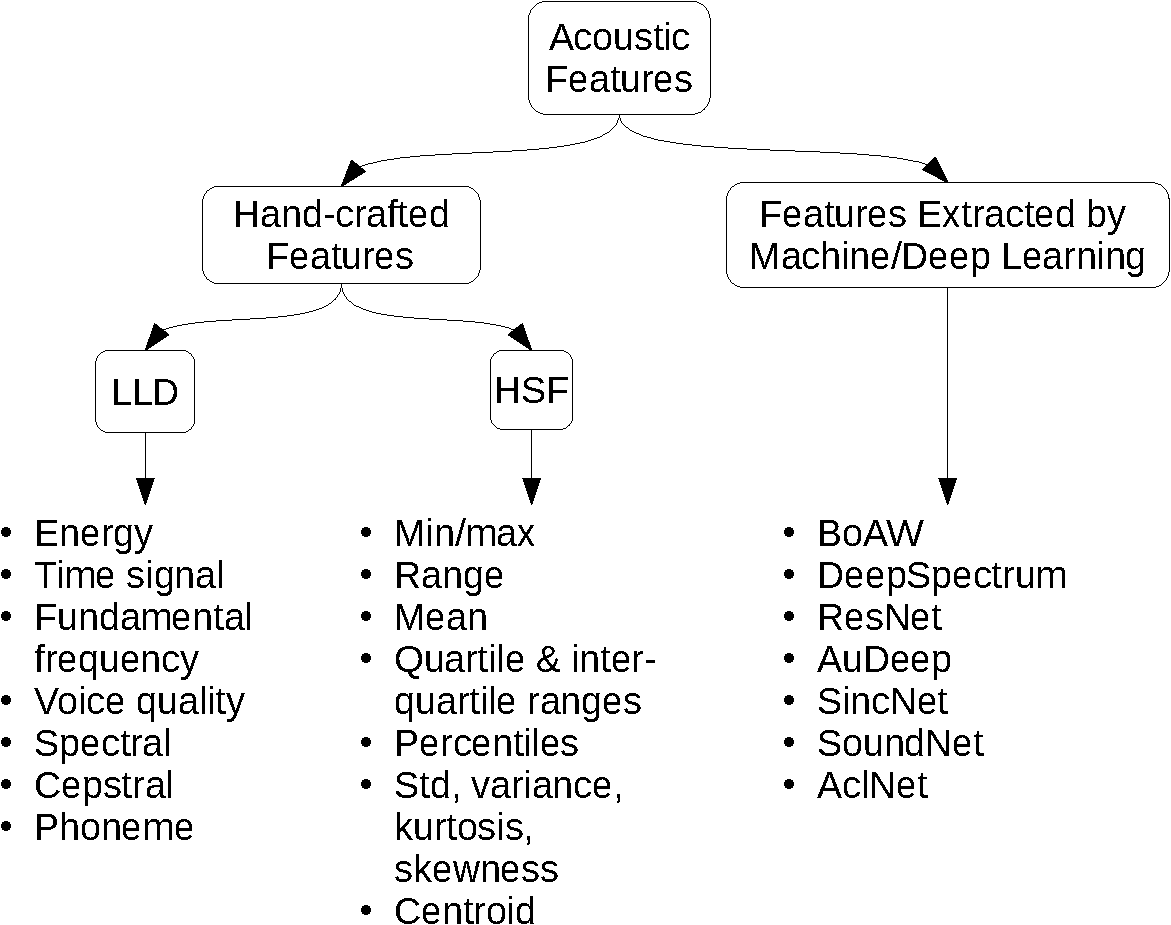
\includegraphics[width=.7\textwidth]{../fig/acoustic_features-crop.pdf}
    \caption{Division of acoustic features for SER}
    \label{fig:aco_feat}
\end{figure}

Eyben et al. \cite{Eyben2010} divided LLD and HSF into five groups: signal
energy, fundamental frequency (perception: pitch), voice quality, cepstral,
time signal, and spectral. Prosodic features ($f_o$, duration, intensity, voice
quality) have been known to have a strong correlation with emotion
\cite{Frick1985,Mozziconacci2002,Fritz2016} from a psychology point of view. In
acoustics, prosody is implemented into several acoustic features, including LLD
and HSF. Vayrynen \cite{Vayrynen2014} made a distinction between prosodic and
acoustic (non-prosodic) features. His study reported that a combination of
prosodic and acoustic features achieved comparable performance to human
reference on basic emotion recognition.

Both references \cite{Lee2002} and \cite{Schuller2004} employed $f_o$ and
energy-based acoustic features for SER. The former applied both LLD and HSF of
$f_o$ and energy features, while the latter only applied HSF of $f_o$ and energy
features. The latter reference found that $f_o$-based features correlated to
SER performance more than energy-based features.

As a `default' feature on most automatic speech recognition (ASR), MFCC has
been explored for SER. Metze et al. \cite{Metze2009} has found that MFCC is the
most informative acoustic features compared to other evaluate acoustic
features. Tripathi et al. \cite{Tripathi2019} found that MFCC performed better
than spectrogram features on unimodal acoustic SER. 

The shift from MFCC to mel-filterbank (MFB) features in ASR motivates SER
researchers to adopt a similar direction. Aldeneh et al. \cite{Aldeneh2017}
extracted 40 MFB features for dimensional SER tasks on the IEMOCAP dataset.
Zhang et al.  \cite{Zhang2019} employed a similar MFB with 40-dimensional with
z-normalization on categorical IEMOCAP and MSP-IMPROV datasets. Both research
showed fair performances (50\% -- 65\% accuracy) from MFB features for the SER
task.

Phoneme, the smallest unit of speech, has been investigated to be useful for
SER task. Zhang et al. \cite{Zhang2019} furthermore combined MFB with phoneme
for the same SER task. A combination of phoneme with MFB outperforms MFB-only
of phoneme-only input features. Yenigalla et al. \cite{Yenigalla2018} combined
phoneme embedding with a spectrogram. The phoneme embedding is generated from
the word2vec model \cite{Mikolov} and IEMOCAP speech data. The combination of
phoneme with spectrogram achieves the highest accuracy among individual
features.

Since most classifiers in modern SER systems used deep learning methods, it is
reasonable to extract an acoustic representation of speech in an end-to-end
manner via deep learning methods. In INTERSPEECH 2020 ComParE challenge, two
deep-learning-based features were given in the baseline system, DeepSpectrum
and AuDeep. The provided DeepSpectrum features with ResNet50 network achieve
the highest unweighted average recall (AUR) on the elderly emotion
sub-challenge test set.

\subsection{Linguistic features}
Linguistic features are the realization of linguistic information. It is also
called text features, textual features, lexical features, language features, or
semantic features. Although linguistic and lexical terms have different
meanings, i.e., language vs. word meaning,  these terms often used
interchangeably in computer science (or information processing). Text features
used in this study also have a different meaning from the same term used in
book or article writing. In book or article writing, the text features include
writing components such as a glossary, bold typeface, title, headings,
captions, and labels. In information science, text or linguistic features are
features extracted from written or spoken text.  Thus, the term linguistic
features is a preferable term than text features to avoid confusion among
readers.

% define a linguistic feature in general
Linguistics features used in emotion recognition represent numerical values
related to the emotional states in a word. The simplest way to build linguistic
features for emotion detection is by emotional keyword spotter
\cite{Chuang2004}. In this framework, every word is assumed to have a
correlation with emotion categories. For instance, the word ``disappointed''
can be represented as [(2, 0.2), (3, 0.6)] where 2 represents ``angry'' emotion
and 3 represent ``sadness'' emotion. Both 0.2 and 0.3 represent degrees of
emotion's intensity. This emotional keyword spotter can be expanded into an
emotional phrase spotter \cite{Schuller2004}.

The first systematic linguistic representation of a document, perhaps, is
TF-IDF (term-frequency inverse document frequency). TF is defined as the
frequency of a word in a particular document/utterance. IDF is defined as a
logarithm of the total number of documents' ratio to the total number
containing that word. TF-IDF is the multiplication of TF with IDF.

Bag-of-Words (BoW) is a numerical feature vector to represent ``words in a bag."
First, a fixed integer is assigned to each word occurring in any documents,
i.e., building a dictionary from a corpus by assigning a word to integer
indices.  Second, count the number of occurrences of each word and store it as
the value of feature $j$ where $j$ is the index of word $w$ in the dictionary
\cite{scikit-learn}.  These BoW features can be expanded for acoustic and
visual modalities (BoAW and BoVW).

Several lexicon dictionaries have been developed to inform the 'emotion score'
of emotional words. These dictionaries include DAL \cite{Whissell2009}, ANEW
\cite{Warriner2013}, VADER \cite{Hutto2014}, and NRC \cite{Mohammad2018}. Using
these dictionaries allows direct measurement of emotional words in the given
utterances. For instance, the word ``arose'' in DAL has values of 2.11, 2.00,
and 1.40 for pleasantness, activation, and imagery. These values are on a
3-point scale; different dictionaries have different scales.

The search for vector representation from a word led to the research of word
embedding or word vector. In this approach, a deep neural network (DNN) is used
to train a large corpus (i.e., a Wikipedia corpus) to generate word vectors
based on an algorithm. This approach has resulted in a new paradigm in the
vector representation of linguistic information of a word. Several models
exist, including word2vec, GloVe, FastText, and BERT. These models are detailed
in Chapter 5.

Figure \ref{fig:ling_feat} shows the division of linguistic features used in
SER task. Similar to acoustic features, there is a tendency to move to deep
learning-based features from hand-crafted features. The choice of linguistic
feature is usually based on the task as in other text processing areas.

% LSA is not mentioned yet
\begin{figure}[htbp]
    \centering
    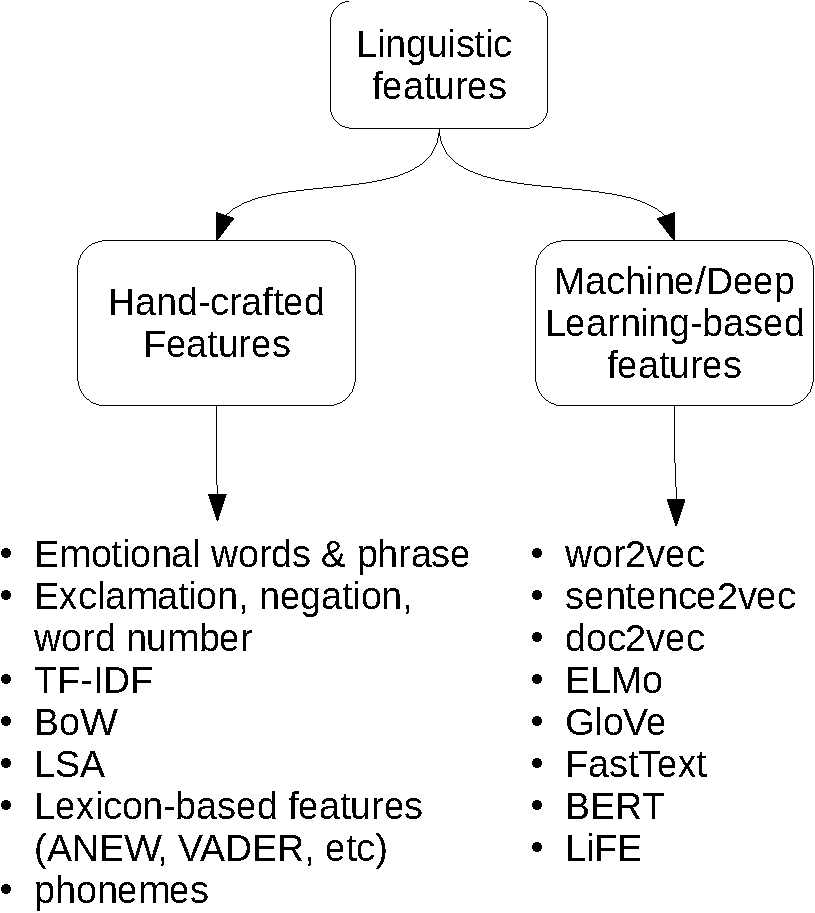
\includegraphics[width=0.6\textwidth]{../fig/linguistic_features-crop.pdf}
    \caption{Divisions of linguistic features used in SER}
    \label{fig:ling_feat}
\end{figure}

% division of linguistic features, list of linguistic features used in SER
% research

% closing statements in Acoustic, most features are hand-crafted features while
% in Linguistics, most features are extracted from deep learning

\section{Classifiers}
This section reviews the four most used classifiers in speech emotion
recognition.  One is a machine learning classifier, i.e., support vector
machine (SVM). Others are three deep learning classifiers, i.e., multilayer
perceptron (MLP), convolutional neural networks (CNN), and long short-term
memory (LSTM) neural networks. The brief descriptions of these classifiers are
given below.

\subsection{SVM}
SVM is a useful machine learning classifier for, generally, small datasets. For
categorical emotion recognition, SVM applies acoustic or linguistic features
for the given labels.  This SVM applied to the classification task is called
support vector classification (SVC).  For dimensional emotion recognition, SVM
applies regression analysis to map them to the given labels. This SVM for
regression task is called as support vector regression (SVR).

SVM can accept unimodal or multimodal inputs. In bimodal emotion recognition
from acoustic and linguistic information, SVM can be utilized in two-stage
scheme for evaluation of the emotion recognition system from DNNs outputs. In
bimodal information fusion, each prediction from the acoustic and text networks
is fed into the SVM.  From two values (e.g., valence predictions from the
acoustic and text networks), the SVM learns to generate a final predicted
degree (e.g., for valence). The concept of using the SVM as the final
classifier can be summarized as follows.

Suppose that two valence prediction outputs from the acoustic and text
networks, $x_i = [x_{ser}[i], x_{ter}[i]]$, are generated by the DNNs, and that
$y_i$ is the corresponding valence label. The problem in dimensional SER fusing
acoustic and text results is to minimize the following: 

\begin{equation}
\begin{aligned}
& \underset{w, b, \zeta, \zeta^*}{\text{min}}
& & \frac{1}{2} w^Tw + C \sum_{i=1}^n \zeta_i + C \sum_{i=1}^n \zeta_i^* \\
& \text{subject to}
& & w^T \phi (x_i)+b- y_i \leq \epsilon  + \zeta_i, \\
&&& y_i - w^T \phi (x_i) -b \leq \epsilon + \zeta_i^*, \\ 
&&& \zeta_i, \zeta_i^* \geq 0, i = 1, \ldots, n,
\end{aligned}
\end{equation}
where $w$ is a weighting vector, $C$ is a penalty parameter, $\zeta$ and
$\zeta^*$ is the distance between misclassified points and the corresponding
marginal boundary (above or below). Here, $\phi$ is the kernel function. On
the use for late fusion approach, the study choose a radial basis function
(RBF) kernel because of its flexibility to model a nonlinear process with a
dimensional emotion model close to this kernel. The function $\phi$ for the RBF
kernel is formulated as: 

\begin{equation}
 K(x_i, x_j) = e^{\gamma(x_i - x_j)^2},
 \label{tab:label}
\end{equation}
where $\gamma$ defines how much influence a single training has on the model.
All parameters in this SVM are obtained empirically via linear search in a
specific range. Although the explanation above uses valence, the same also
applies for arousal and dominance. 

% add literature review for SVM

\subsection{MLP}
MLP is a classical feedforward neural network by projecting input data into
linearly separable space using non-linear transformation. A hidden layer is an
intermediate layer between inputs and outputs, containing many perceptrons
(also called units or nodes). An MLP commonly refers to more than one hidden
layer. The MLP used here is similar to the definition of connectionist learning
proposed by Hinton \cite{Hinton1989}. A deeper layer MLP usually consists of
many layers to enable deep learning hierarchically. This neural network
architecture is also known as dense network or fully-connected (FC) network.
  
% parameter
MLP is a simple yet powerful tool for combining acoustic and linguistic
information via network concatenation. Mathematically, the combined
acoustic+linguistic network could be formulated as in equation \ref{eq:mlp}.
Here, $f(y)$ denotes the output of the corresponding layer; $W_1, W_2$ denote
the weights from previous layers ($a$: acoustic; $l$: linguistic), i.e., a dense
layer after LSTM for each network, and the current hidden layer, respectively;
$x_a$ and $x_l$ are the acoustic features and word embeddings, respectively;
$b$ is a bias; and $g$ is an activation function. Thus, the output of the that
dense layer is 
\begin{equation}
f(y) = W_2 g ([W_{1a}^\top xa + b_{1a};W_{1l}^\top xl + b_{1l}]) + b_2
\label{eq:mlp}.
\end{equation}

Schuller et al. \cite{Schuller2004} utilized MLP for combining acoustic and
linguistic information. Their evaluation using MLP showed lower error than the
fusion method by means of logical ``OR''. Callejas and L\'opez-C\'ozar
\cite{Callejas2008} compared baseline majority-class method to MLP for
evaluating the effect of context information on categorical SER task. The
result shows that MLP outperforms the baseline method in six out of eight
scenarios. Zhang et al.  \cite{Zhang2019} used MLP in all experiments involving
acoustic features, phoneme, and combination of both; MLP showed its
effectiveness on both single-stage and multi-stage SER tasks.

% add literature review for MLP

\subsection{CNN}
% review cnn here, take the theory from d2l.ai, refer to CNN in SER paper.
CNN is a class of neural networks that contain a convolutional layer.
Convolution is a mathematical operation between two functions by measuring the
overlap of both when one function (``input'') is flipped and shifted by another
function (``kernel''). The resulting output, which is the goal of a convolution
layer, is a feature map. This convolution operation is similar to
cross-correlation; cross-correlation does not flip the second function.
Convolution is also can be seen as cross-correlation with a scalar bias. In
deep learning literature, the convolution terminology views cross-correlation
as convolution since many deep learning frameworks did not take bias into
account by default. 

The convolutional network is often applied to image-like data. Time-series
data, including acoustic feature vector, can be fed into convolutional networks
using 1-dimensional (1D) CNN. To take the most benefit of CNN, spectrogram and
mel-filterbank (MFB) features are frequently used to input the SER system. For
text processing, the main idea for CNN is to compute vectors for n-gram (e.g.,
2-, 3-, and 4-gram) and group them afterward. CNN is commonly used for both
speech and language processing. 

Apart from convolutional layers, CNN typically still needs a fully-connected
layer (FC or MLP). The feature map as the output of the convolution layer is
fed into MLP to obtain desired outputs. Although recently it is found
unnecessary \cite{Springenberg2015}, a CNN commonly uses pooling layers after
convolutional layers for mitigating and reducing spatial representation
\cite{Zhang2020}.

Yenigalla et al. \cite{Yenigalla2018} experimented with CNN for categorical
SER by inputting phoneme, spectrogram, and combination of both. The combination
of both phoneme embeddings and spectrogram achieved the highest performance.
The architecture of each phoneme and spectrogram networks was convolution layer
and max-pooling and FC layer. Both networks are concatenated by FC layers
to obtain the outputs.

Instead of phoneme and spectrogram, Huang et al. \cite{Huang2018} proposed to
use bag-of-audio-words for the input of the CNN-based SER system. The
architecture was similar to \cite{Yenigalla2018}, i.e., convolution, pooling,
and FC layer.  The result shows that the use of BoAW outperforms raw acoustic
features.

Cho et al. \cite{Cho2018} combined acoustic and linguistic information for
categorical SER; the acoustic inputs used an LSTM network while the linguistic
inputs used a multi-resolution CNN. A multi-resolution CNN is utilized to
emotion words by employing word embedding, convolution layer, and global mean
pooling. The combination of acoustic network with LSTM, linguistic network with
CNN, and emotion vector (e-vector) achieved the highest performance compared to
unimodal results.

While most bimodal SER research used CNN for linguistic and LSTM for acoustic
information processing, Sebastian and Pierucci \cite{Sebastian2019}, used LSTM
for text and CNN for speech. The CNN architecture contains two convolution
layers and two FC layers. In this case, the performance of CNN-based text
emotion recognition is the lowest among other models.


Cai et al. \cite{Cai2019} replaced FC layers in most CNN architectures with
bidirectional LSTM with attention. The improved architecture was called
CNN-Bi-LSTM-Attention (CBLA). On both unimodal and multimodal, CBLA outperforms
MLP models by considering both global and temporal information in the data.

\subsection{LSTM}
Long Short-Term Memory (LSTM) neural networks is an extension of a recurrent
neural network. The idea of using LSTM networks comes from an approach that
human has the persistence to keep memory long in a short-term period. Humans do
not start their thinking from scratch every second. When reading a paper, a
reader understands each word based on the understanding of the previous words.
Humans do not throw everything away and start thinking from scratch again. The
thoughts have persistence.

Three gates are introduced in LSTMs: the input gate ($\mathbf{I}_t$), the
forgetting gate ($\mathbf{F}_t$), and the output gate ($\mathbf{G}_t$). In
addition to that we introduce memory cells that take the same shape as the
hidden state.  A memory cell is just a fancy version of a hidden state, custom
engineered to record additional information. The three gates in LSTM are
defined as:

\begin{align}
\mathbf{I}_t &= \sigma(\mathbf{X}_t \mathbf{W}_{xi} + \mathbf{H}_{t-1} \mathbf{W}_{hi} + \mathbf{b}_i),\\
\mathbf{F}_t &= \sigma(\mathbf{X}_t \mathbf{W}_{xf} + \mathbf{H}_{t-1} \mathbf{W}_{hf} + \mathbf{b}_f),\\
\mathbf{O}_t &= \sigma(\mathbf{X}_t \mathbf{W}_{xo} + \mathbf{H}_{t-1} \mathbf{W}_{ho} + \mathbf{b}_o).
\end{align}

Then the candidate memory cell, memory cell, and hidden state are calculated on
the following equations:

\begin{align}
\widetilde{C}_t &= \text{tanh}(\mathbf{X}_t \mathbf{W}_{xc} + \mathbf{H}_{t-1} \mathbf{W}_{hc} + \mathbf{b}_c), \\
\mathbf{C}_t &= \mathbf{F}_t \odot \mathbf{C}_{t-1} + \mathbf{I}_t \odot \tilde{\mathbf{C}}_t, \\
\mathbf{H}_t &= \mathbf{O}_t \odot \tanh(\mathbf{C}_t).
\end{align}

Graphical illustration of LSTM explained by equations above is shown in Figure
\ref{fig:lstm}.

\begin{figure}[!hb]
\centering
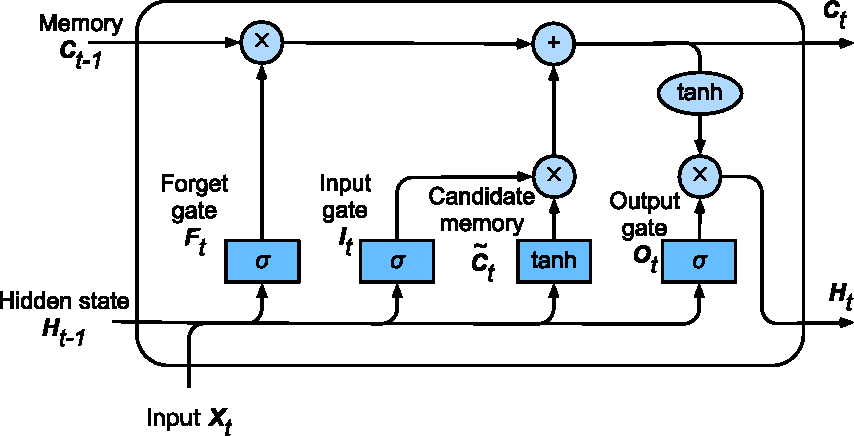
\includegraphics[width=4.5in]{../fig/lstm_3.pdf}
\caption{Graphical illustration of LSTM \cite{Zhang2020}}
\label{fig:lstm}
\end{figure}

% add literature review for LSTM
LSTM has dominated the classifiers used in both ASR and SER. Since the data
(i.e., input features) are sequence, a recurrent neural network is a
straightforward way to process these data. In addition, LSTM is able to model
long-range context in emotional features to map it with the emotional labels.
Tian et al. \cite{Tian2015} used the LSTM classifier to build hierarchical
neural networks. In \cite{Cho2018}, LSTM was used to train acoustic features
before the network was concatenated with a CNN-based linguistic network.

Instead of unidirectional LSTM, bidirectional LSTM (BLSTM) has been utilized to
learn information both from the past and the future inside the network
(unidirectional LSTM only learns from the past). In \cite{Cai2019}, BLSTM is
used for the textual network rather than the acoustic network. This
bidirectional LSTM is often combined with an attention model to boost the
performance of the SER task \cite{Atmaja2019}. However, using BLSTM doubles the
model's complexity, making the model may be not suitable for real-time
applications.

\section{Fusion Methods} 
Multimodal fusion in technology is the combination of information that comes
from different sources \cite{Khaleghi2013}. This terminology is similar but
different to the human multimodal perception. In human multimodal perception,
the information comes from different sensory organs; in technology, this
requirement is not necessary.  Multimodal fusion can be viewed as multisensor
data fusion. In this terminology, the `sensor' is the soft sensor. Acoustic and
linguistic feature extractors can be regarded as soft sensors in bimodal
acoustic-linguistic information fusion.

Fusing acoustic and linguistic features have been attempted at the early stage
of speech emotion recognition research. The first work on fusing acoustic with
linguistic information has been performed by Lee et al. \cite{Lee2002} by
combining acoustic and language features at the decision level using logical
``OR''. If at least one decision corresponds to a specific emotion, then the
result is this specific emotion. This earliest work only involved negative and
non-negative emotion categories.

Fusing acoustic and linguistic information for SER can be accomplished in
several ways, Figure \ref{fig:ser_bimodal} shows the classification. Early
fusion combines acoustic and linguistic information at the feature level; late
fusion combines results from acoustic and linguistic information at the
decision level.  Early fusion, furthermore, can be split into three main
categories: feature concatenation, networks/model concatenation, and
hierarchical model.  Hierarchical model, as proposed in
\cite{Majumder2018,Tian2019}, can be regarded as early fusion since the method
fuses features at a different level of layers, not at the decision level.

\begin{figure}[htbp]
    \centering
    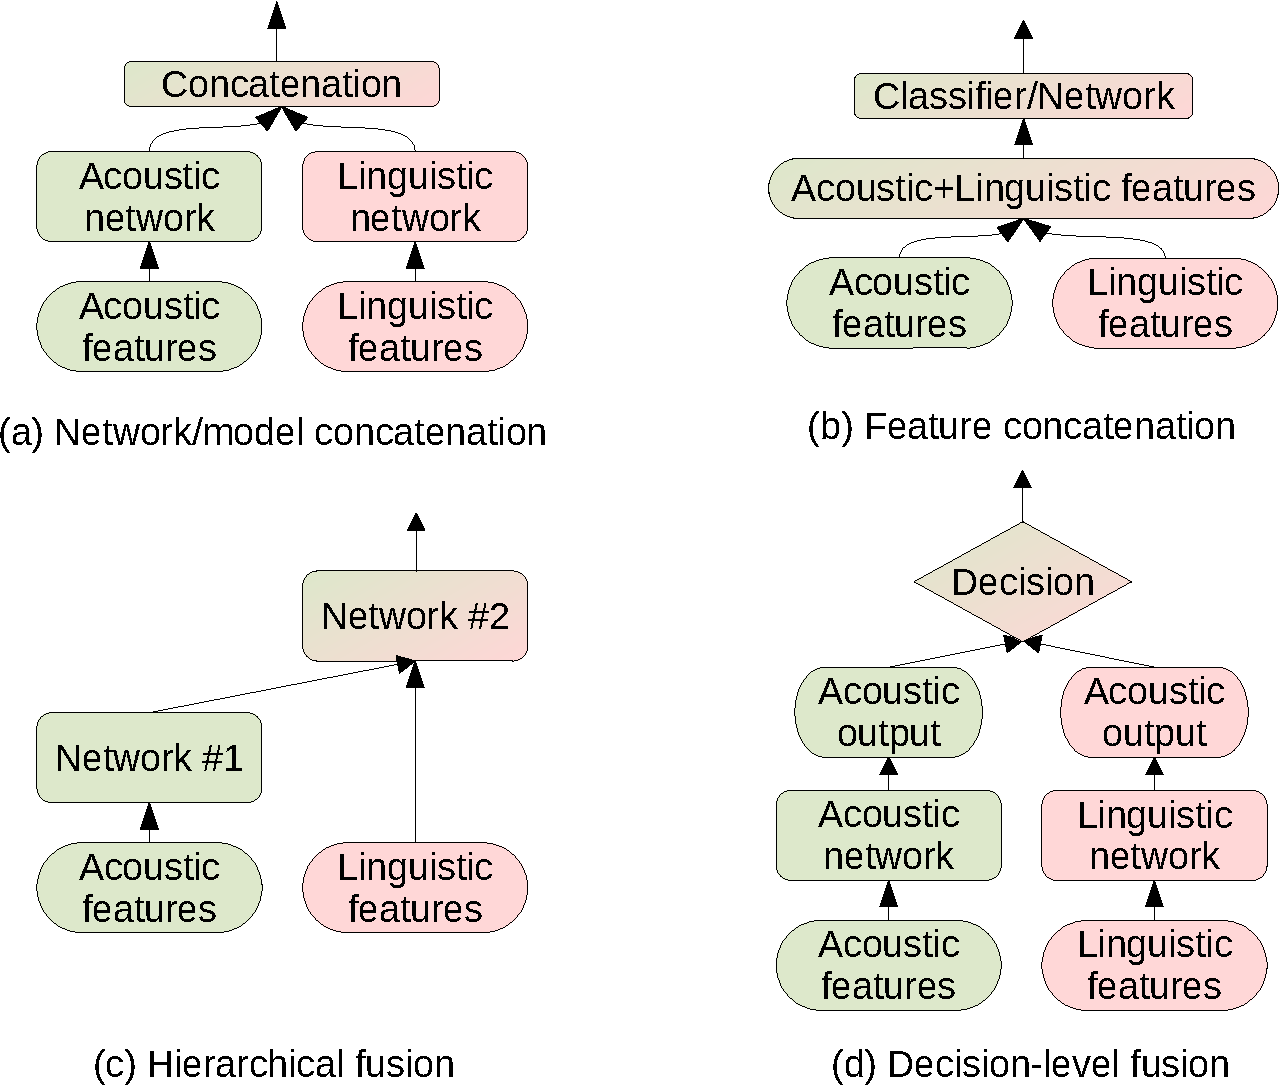
\includegraphics[width=0.9\textwidth]{../fig/ser_bimodal-crop.pdf}
    \caption{Different scheme of fusing acoustic with linguistic information; (a), (b), (c): early fusion approach; (d): late fusion approach}
    \label{fig:ser_bimodal}
\end{figure}

Eyben et al. \cite{Eyben2010} proposed an online method to detect not only
valence and arousal but also the time when those emotion attributes are
detected. They used a recurrent neural network (RNN) based on long short-term
memory (LSTM) to recognize a framewise valence-arousal continuum with time. By
adding a keyword spotter, they were able to improve the performance by using
regression analysis. The results were measured in Pearson correlation
coefficient (PCC).  They also found that keywords like ``again,'' ``angry,''
``assertive,'' and ``very'' were related to activation, while typical keywords
correlated to valence were ``good,'' ``great,'' ``lovely,'' and ``totally.''
Similar to that idea, Karadogan and Larsen \cite{Karadogan2012} used affective
words from Affective Norms for English Words (ANEW) to determine
valence-arousal values and combine them with a result from acoustic features.
The latter paper also obtained similar improvements over any single
modality.

Ye and Fan \cite{Ye2014} used bimodal features from acoustic and text
information to recognize emotion within speech. The acoustic features were
trained in two parallel classifiers: an SVM and a backpropagation network. The
text features were trained in two serial classifiers, which were both Naive
Bayes classifiers.  The second classifier acted as a filter for unreliable
parts from the first classifier. Decision-level fusion (late fusion) was then
implemented by combining the acoustic and text features with tree-weighting
factors for the SVM, backpropagation network, and text classifiers. The
resulting fusion method obtained 93\% accuracy, as compared to 83\% from the
acoustic features only and 89\% from the text features only. The task was
categorical emotion detection from a Chinese database. Similar to that approach
for a categorical task, Jin et al. \cite{Jin2015} used the IEMOCAP dataset to
test combinations of acoustic and text features for SER. The novelty of their
method was the use of an emotion vector for lexical features, which improved
the accuracy in four-class emotion recognition from 53.5\% (acoustic) and
57.4\% (text) to 69.2\% (acoustic + linguistic).

Aldeneh et al. \cite{Aldeneh2017} used acoustic and lexical features to detect
the degree of valence from speech. They used 40 mel-filterbanks (MFBs) as
acoustic features and word vectors as linguistic features. Continuous valence
values were then converted to three categorical classes: negative, neutral, and
positive. Using that approach, they improved the weighted accuracy from 64.5\%
(linguistic) and 58.9\% (acoustic) to 69.2\% (acoustic + linguistic). 

Yoon et al. \cite{Yoon2018} used audio and text networks to predict emotion
classes from the IEMOCAP dataset. Both networks used RNNs with inputs of
mel-frequency cepstral coefficients (MFCCs) for audio and word vectors for
text. The proposed multimodal dual recurrent encoder (MDRE) improved on the
single-modality RNNs from 54.6\% (audio) and 63.5\% (text) to 71.8\% (audio +
text). Atmaja et al.  \cite{Atmaja2019b} obtained a better result by using 34
acoustic features after silence removal and combining them with word
embeddings. With  LSTM used for the text and dense networks for speech, the
latter paper obtained an accuracy of 75.49\% on the same dataset and task
(categorical emotion recognition).

Instead of using lexical features, Zhang et al. \cite{Zhang2019} used phonemes
and combined them with acoustic features to recognize valence in speech. They
used 39 unique phonemes from the IEMOCAP and MSP-IMPROV datasets and a
40-dimensional log-scale MFB energy for the acoustic features. Using a scaled
version of valence, converted from a 5-point scale to three categorical
classes, they showed that their multistage fusion model outperformed all other
models on both IEMOCAP and MSP-IMPROV.

\section{Summary}
This chapter reviews research on bimodal speech emotion recognition from
acoustic and linguistic information. The study focuses on four building blocks
of SER from bimodal information: emotion models, features, classifiers, and
fusion methods.  There are three emotion models developed in psychological
research; however, most SER research focused on the categorical model. There is
a move to extract acoustic features in the feature extraction step by using
deep-learning methods, while deep-learning-based linguistic features already
dominated text processing research, including SER from linguistic information.
Four common classifiers for SER are briefly described.  Although more advanced
DNN architectures have been developed, bimodal SER still relies heavily on SVM,
MLP, CNN, and LSTM architectures. Finally, the fusion of different information
can be performed in several methods; these methods can be divided into early
and late fusions. While this literature study presents the current state of
speech emotion recognition research in these four blocks, the raised issues in
SER research will be highlighted in the next Research Methodology chapter along
with other related sections. 

\chapter{Research Methodology}

The purpose of this chapter is to introduce the research methodology, the
justification for using particular research methods used in this experimental
study on dimensional speech emotion recognition by fusing acoustic and
linguistic information. This approach allows the examination of the
contribution of fusing bimodal information for more accurate dimensional speech
emotion recognition. The research issues and philosophies used to tackle these
issues are discussed in this chapter. The implementation of research philosophy
through research strategies are highlighted. The experimental methods,
including datasets and an evaluation metric, are also the primary components of
the research methodology presented to close this chapter.

\section{Research motivation}
\subsection{Why is SER difficult?}
Speech emotion recognition (SER) is a difficult task. It differs from other
traditional tasks like image recognition (cat vs. dog), digit recognition, or
speech recognition. For instance, the features and labels for recognizing cat
or dog in image recognition are both clear. The difference in eyes, ears, skin
color, and shape between cat and dog can be used as informative features. The
labels also clear, either cat or dog, with a very high level of confidence. The
digit recognition problem has similar properties; from zero to nine can be
distinguished by their shapes; this input feature is an important factor for
the obtaining high accuracy classification.  Automatic speech recognition (ASR)
also has similar properties to both cases. SER is different from both cases.   

In SER, both features and labels are not clear. Researchers have attempted to
find useful features related to affective states (e.g.,
\cite{Batliner2011,Mairano}). In annotating labels for categorical or
dimensional emotion, the datasets makers rely on subjective evaluation. This
means that the labels are not exact values (e.g., compared to image labels).
However, high agreements among evaluators show the reliability of the datasets.
In this SER problem, it is almost impossible to obtain perfect accuracy, which
is possible to obtain in the previous image recognition problems.

\subsection{Why study dimensional SER?}
% argue with Darwin position
While most SER research focus on categorical emotion recognition, only a few
focuses on dimensional SER. In contrast, the present evidence about the
``fingerprint'' in categorical emotion, particularly based on facial
expression, is weak \cite{Barrett2019}. As Darwin argued that biological
categories, including emotion categories, does not have an essence due to the
high variability of individuals \cite{charles1872expression}, so does emotion
categories. 

Dimensional emotion may represent humans' affective state better than
categorical emotion. Humans do not perceive emotion categorically but in
continuous space. In this case, Russell argued that emotion categories could be
derived from valence-arousal space \cite{Russell1980}. Given this understanding,
dimensional SER is more challenging (since it predicts degree) and more useful
(since categorical emotion also can be derived) than categorical emotion
recognition.

% adding supporting research from "four not six" adding supporting factor from
% newest emotion model

\subsection{Why fuse acoustic with linguistic information?}
The third motivation is about the use of linguistic information. The simplest
answer to this question is that linguistic information is also can be extracted
from speech, and language is related to emotion. In other words, two pieces of
information can be extracted from speech without adding other modalities to
recognize expressed emotion. Hence, fusing acoustic and linguistic information
is reasonable and feasible for future SER implementation.

% other reasons: human multimodal processing and sentiment analysis
There are other possible motivations for fusing acoustic and linguistic
information for dimensional SER. One is from human multimodal processing, which
uses linguistic information as a cue for emotion perception
\cite{Lindquist2006}.  Another reason is that linguistic information is widely
used in sentiment analysis tasks, which are closely related to emotion
recognition. Sentiment analysis can be viewed as emotion recognition in text,
which focuses on sentiment or valence prediction.

% speech is basic need and may less private than image and video Speech is the
% most fundamental way to communicate. People use their voice to communicate,
% share experience, exchange ideas or transmit knowledge
% \cite{denes1993speech}. In some cases, people cannot avoid using speech to
% solve their urgent needs, e.g., complaining about a problem or calling a
% relation or a call center. Due to this necessity (to communicate with
% others), speech (acoustic and linguistic information) may less private than
% image or video data. 

In the speech chain, acoustic and linguistic are connected by a physiological
mechanism \cite{denes1993speech}. This chain shows a direct correlation between
linguistic and acoustic information. Fusing both pieces of information may
improve the prediction of the conveyed message. Since the message is elicited
from the same sources (e.g., thought, information, including emotion), using
both pieces of information is a straightforward way to track the transported
information, in this case, the expressed emotion of a speaker.

\section{Research issues}
% all issues
There are five issues discussed in this dissertation. The issues appeared from
the previous SER studies \cite{ElAyadi2011, Li2019b}. These issues raised in SER
from acoustic information, dimensional SER, and multimodal SER. Although these
issues are important, the previous chapter on literature study has found no
thorough study investigated on these five issues. The importance of these issues
and the contributions of this study to these issues are summarized below.

The first issue is the region of analysis used for feature extraction in
dimensional SER, local areas in frames, or whole utterance processing. The
importance of addressing this issue is to determine which region of analysis is
informative to extract dimensional emotion from speech. The
traditional way to extract acoustic features in acoustical signal processing is
frame-based processing. In this way, an utterance is split into several frames
in a fixed duration, e.g., 25 ms. A window function applies to these frames,
and the intended acoustic features are extracted on these frames. This local
feature extraction is known as a low-level descriptor (LLD). In contrast, the
newer research on speech emotion recognition proposed to extract statistical
functions based on these LLDs. These global features are known as high-level
statistical function (HSF). Form both features, it is unclear which one
performs better; one claimed that LLDs are enough since it is highly correlated
with emotion (e.g., tone and prosody \cite{Fritz2016}), others claimed that
global features are better in classification accuracy and classification time
(perhaps due to small feature size) \cite {ElAyadi2011}. This study revealed the
significant contribution of specific method for solving the effectiveness of
region analysis for acoustic feature extraction.

The second issue is the effect of the silence region in dimensional speech
emotion recognition. This issue is important to know whether such
post-processing techniques contribute to dimensional SER. In conventional ways,
acoustic features are extracted from speech utterance, including the silence
region. Some removed silence before extracting acoustic features (e.g.,
\cite{Atmaja2019, Elbarougy2019, Mairano, Aguilar2020}) and some used silence
as a feature (e.g., \cite{Atmaja2020f, Tian2015a}) or as an emotion category
\cite{Fayek2017}. Although silent pause is an important cue for human speech
communication \cite{Ephratt2008, Tisljar-Szabo2014}, it is unclear whether
silence contributes to human-computer communication (HCI). This study
contributed to this effect of silent pause region by predicting the role of the
region to dimensional SER.

The third issue is the low score of valence prediction in dimensional SER.
Among the three emotion dimensions, valence always obtained lower scores than
arousal and dominance. The previous study confirms this evidence
\cite{Li2019b}.  Considering valence is the most important emotion dimension
\cite{Fontaine2017}, the need to improve valence prediction score is worthwhile
to study. Although there are several attempts to improve valence prediction
\cite{Zhang2019, Aldeneh2017,Sridhar2018}, the obtained scores are still not
comparable to the scores achieved by arousal and dominance (e.g., in
\cite{Sridhar2018}). This study proposed and discussed a method to double the
performance of valence prediction in dimensional SER.

The fourth issue is whether it suffices to use acoustic features for modeling
emotions or if it is necessary to fuse them with linguistic features. Since
linguistic information can be obtained from speech (via ASR), it is reasonable
to fuse linguistic information with acoustic information. In HCI, the simplest
method to fuse multimodal information is by concatenating input features from
all modalities. More improvisation can be performed by concatenating models
instead of features. In other study, it was found that linguistic information
helps to improve valence prediction \cite{Karadogan2012}. Fusing acoustic and
linguistic information may improve not only valence prediction but also other
emotion dimensions. This study reveals the necessity of fusing both acoustic
and linguistic information for dimensional SER.

The fifth issue is the scheme or framework to fuse linguistic and acoustic
information. If the linguistic information contributes to dimensional emotion
prediction, what the most appropriate approach to fuse acoustic and linguistic
information is. In human multimodal emotion perception, how multimodal
information are fused is not clear yet. Both acoustic and linguistic
information are believed to be processed separately in different regions of the
cortex (right and left hemisphere). This mechanism inspires the late fusion
approach by processing each modality separately and fusing both results at the
decision level. This study showed the effectiveness of late fusion approach
over early fusion approach for combining acoustic and linguistic information
for dimension SER.


\section{Research philosophy}
Research philosophy can be defined as ``a belief about the way in which data
about a phenomenon should be gathered, analyzed and used \cite{Davison1998}."
This research used data-information-knowledge hierarchy (DIK) concept, which is
known as the canon of information science \cite{Fricke2009}. Figure
\ref{fig:research_concept} shows this DIK concept and its representation in the
speech emotion recognition area. Although some researchers defined these
concepts in different ways \cite{Badia2013, Liu2013}, the following concepts
are the proper and valid explanation used in this research.
% Human multimodal information fusion is unclear until now

% Human emotion perception The human ability to imagine situations in detail
% comes from the right hemisphere of the cortex, which approaches the world
% differently than the analytical, verbal left hemisphere. The right hemi-
% sphere is nonverbal and processes things in more holistic, integrated ways.
% It helps us see patterns, recognize faces, and identify and express emotions
% (Rewriting ...)

% change the picture to triangle (DIK) with its representation Speech, Acoustic
% + Linguistic, Emotion

% \subsection{}
\begin{figure}[htbp]
    \centering
    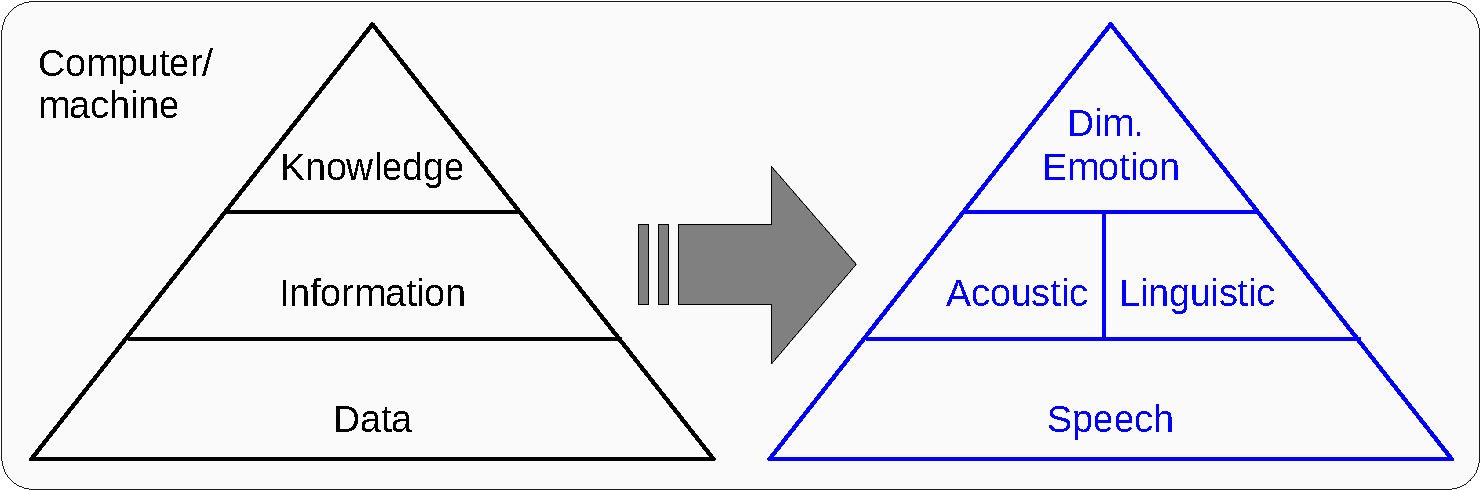
\includegraphics[width=.8\textwidth]{../fig/DIK_SER-crop.pdf}
    % \caption{A concept used in this research: acoustic and linguistic
    % information are extracted from (speech) data to obtain knowledge -- the
    % dimensional emotion.}
\caption{The DIK hierarchy and its representation in speech emotion
recognition; information (I) is extracted from data (D); knowledge (K) is
extracted from information.}
    \label{fig:research_concept}
\end{figure}

\subsubsection{Data: speech}
Data is worth nothing. According to Choo \cite{Choo2007}, signals structure the
data. Acoustic signal composes speech; speech is the data. In human
communication, speech by a speaker is data for the listener. In HCI, the speech
dataset is a collection of recorded utterances from speakers elicited intended
expressions. An emotional speech dataset is a type of speech dataset that
provides utterances with their emotional labels in categorical or/and
dimensional emotions.

\subsubsection{Information: acoustic and linguistic}
Information is know-what. It is the relevant, usable, significant, meaningful,
or processed data \cite{Rowley2007}. Information is extracted from data. Humans
arguably perceive the speaker's emotions from their acoustic and linguistic
information \cite{Nygaard2008}. How both pieces of information fused is not
clear until now; however, researchers suggest that both perceived information
are processed separately \cite{Berckmoes2004, Kotz2011}, verbal information in
the left cortex and non-verbal information in the right cortex. In HCI,
acoustic information can be extracted directly from speech, while linguistic
information needs a mediator, i.e., speech-to-text system, to extract words
from speech. Then, linguistic information can be extracted from these words.
Both pieces of information are represented as features. Feature extraction is
the process of extracting acoustic and linguistic information from the speech
dataset and its transcription.

\subsubsection{Knowledge: dimensional emotion degrees}
Knowledge is know-how. It is extracted from the information. Knowledge
transforms information into instructions. In human communication, the knowledge
to perceive emotion is innate rather than learned \cite{Matsumoto2009}. In
dimensional emotion, the outputs of this knowledge are the degrees of valence
(V), arousal (A), and dominance (D) [e.g., V=4, A=4, D=2]. The process of
mapping information (features) to dimensional emotion degree is a regression
task which is performed by such regressors. 

\section{Research strategy}
A research strategy is the steps or ways in which research's goals could be
achieved. The goal of this study is to answer the research issues presented
previously. This research investigates three strategies to answers these
research issues. The following are the description and rationale of the
strategies.

% outline three proposed methods, which methods to tackle which issues
\subsection{Dimensional SER by acoustic information}
This study evaluated dimensional SER based on acoustic features to tackle the
first and second issues.  This study aims at maximizing the potency of
acoustic-based SER. First, the region of analysis is investigated. A thorough
comparison among three conditions are performed: (1) extracting acoustic
features from silence-removed regions, (2) extracting acoustic features from
the whole region, including silence, and (3) extracting features from the whole
region and utilizing a silence feature as an additional feature. Second, this
study evaluated which aggregation method performs better: input features
aggregation or outputs aggregation. The common approach in aggregation is
output aggregation by majority voting; however, input aggregation may perform
better, particularly dimensional SER. For instance, humans may perceive emotion
from acoustic information aggregation (e.g., tones) to recognize the emotion
based on that information (rather than aggregating emotions/outputs). As found
in other SER research, this study contributes to the necessity to go beyond
acoustic-only SER.

% add fictitious case where linguistics may helps
\subsection{Fusing acoustic and linguistic information at feature level}
In certain cases, it may be difficult for a listener to perceive the speaker's
emotion from acoustic information only. For instance, both joy and angry may
have a similar intonation (e.g., high tones); hence it is difficult to
differentiate both emotions. By knowing the semantic of utterances, it may be
easier to judge the expressed emotion for both human-human communication and
human-computer communication.  This case raises an opportunity to investigate
whether linguistic information contributes to dimensional emotion recognition.
Although the study of this phenomenon has been performed previously (e.g., in
\cite{Karadogan2012}), several limitations still exist. The emotion model, the
used linguistic information, and the classification framework have evolved
since the publication.

Apart from the need for multimodal/bimodal information fusion, linguistic
information has been actively developed for sentiment analysis, analyzing text
to obtain the affective state of the writer (positive or negative).  This
`sentiment' term reflects directly to valence; hence, one possible solution to
improve low valence score in dimensional SER is by utilizing linguistic
information. Research showed that utilizing linguistic information improves
both categorical {\cite{ Yoon2018} and dimensional \cite{Karadogan2012} emotion
recognitions. Fusing acoustic and linguistic information tackles both the third
and fourth issues: the low score valence prediction and the necessity of using linguistic information.

A simple approach to fuse acoustic and linguistic information is by fusing both
at the feature level. In this approach, either features or networks can be
concatenated to predict dimensional emotions. In the first method, all features
are inputted to the same classifier, while in the latter, both pieces of
information may have different classifiers (networks). In the latter method,
additional networks are needed to fuse both networks, typically a type of dense
networks (also called as fully connected [FC] networks or multilayer perceptron
[MLP]).

Although there are several studies that focus on the linguistic and acoustic
features fusion for SER at the feature level, this study differs in several
aspects. First, this study evaluated both feature concatenation and network
concatenation. Second, this study proposed correlation-based multitask learning
(MTL) to predict valence, arousal, and simultaneously from both acoustic and
linguistic information. Third, this study contributes to a comparison of manual
and automatic transcriptions for acoustic-linguistic dimensional SER.

\subsection{Fusing acoustic and linguistic information at decision level}
To extend the fourth issue, it is necessary to study the fusion of acoustic and
linguistic information not only at the feature level but also at the decision
level. This strategy is motivated by human multimodal processing. The neural
mechanism on how the brain processes multimodal information suggests that each
information is processed in a separate brain region. Hence, a late fusion
approach, i.e., decision-level information fusion, may work better than
feature-level fusion. Apart from investigating which fusion method is better to
combine bimodal information (the fifth issue), this strategy can also be used
to investigate the third and fourth issues.

This last strategy contributes to investigate which framework performs better
for fusing acoustic and linguistic information. Although there is an argument
that any fusion approach will perform similarly \cite{Pepino2020}, the opposite
also has been argued \cite{Planet2012}. Consistency found in this study (that
late fusion is better than early fusion) may help the future research on
dimensional SER and trigger more ways to fuse both acoustic and linguistic
information for SER.

% \section{Experiments}
\section{Datasets}
The strategies to answer research issues need several instruments to experiment
with. One key component in this dimensional SER research is dataset. Three
emotional speech datasets have been chosen for different experiments. These
three datasets are explained below. \\

% explain three datasets and their partition
\noindent 1. IEMOCAP \\
IEMOCAP, which stands for interactive emotional dyadic motion capture database,
contains dyadic conversations with markers on the face, head, and hands. The
recordings thus provide detailed information about the actors' facial
expressions and hand movements during both scripted and spontaneous spoken
communication scenarios \cite{Busso2008}. This research only uses acoustic and
linguistic features because the goal is bimodal speech emotion recognition. The
IEMOCAP dataset is freely available upon request, including its labels for
categorical and dimensional emotions. This study uses dimensional emotion labels
(valence, arousal, dominance), which are average scores for two evaluators,
because they enable deeper emotional states analysis. The dimensional emotion
scores, for valence, arousal, and dominance, are meant to range from 1 to 5 as
a result of Self-Assessment Manikin (SAM) evaluation. It has been found that
some labels with scores lower than 1 or higher than 5. Either removing those
data (seven samples) or converting them into neutral (a score of 3) was chosen
in different experiments.  All labels are then converted from the 5-point scale
to a floating-point values range [-1, 1] when fed to a DNN system.

The total length of the IEMOCAP dataset is about 12 hours, or 10039
turns/utterances, from ten actors in five dyadic sessions (two actors each).
The speech modality used to extract acoustic features is a set of files in the
dataset with a single channel per sentence. The sampling rate of the speech
data was 16 kHz. The manual transcription in the dataset without additional
preprocessing is used for text data except for comparing it with ASR outputs
(chapter 5). \\

\noindent 2. MSP-IMPROV \\
MSP-IMPROV \cite{busso2016msp}, developed by the Multimodal Signal Processing
(MSP) Lab at the University of Texas, Dallas, is a multimodal emotional
database obtained by applying lexical and emotion control in the recording
process while also promoting naturalness. The dataset provides audio and visual
recordings, while text transcriptions are obtained via automatic speech
recognition (ASR) provided by the authors of the dataset. As with IEMOCAP, the
speech and speech+text data with dimensional emotion labels were used in
different experiments. The annotation method for the recordings was the same as
for IEMOCAP, i.e., SAM evaluation, with rating by at least five evaluators.
Some data with missing evaluations were treated as neutral speech (i.e., a
score of 3 for valence, arousal, and dominance). Also, as with IEMOCAP, all
labels are converted to floating-point values in the range [-1, 1] from the
original 5-point scale.

The MSP-IMPROV dataset contains 8438 turns/utterances in more than 9 hours.
Similar to IEMOCAP, there are two speakers for each session. The number of
sessions is six. Originally, the dataset is divided into four scenarios:
``Target-improvised" and ``Target-read," ``Other-improvised," and
``Natural-interaction.'' This allotment was designed to evaluate the effect of
target sentences. The whole dataset is used for acoustic-only emotion
recognition. The parts of MSP-IMPROV, excluding ``Target-read," are used for
acoustic-linguistic information fusion. A further explanation about this
dataset will be added in the explanation of the experiment involving this
dataset (Chapter 6).\\

\noindent 3. USOMS-e \\
Ulm State of Mind in Speech-elderly (USOMS-e) dataset is the corpus used in the
elderly emotion sub-challenge in the INTERSPEECH 2020 computational
paralinguistic challenge. The whole dataset subset is used with 87 subjects
aged 60 -- 95 years; 55 of the subjects were male, and the rest 32 were female.
The dimensional emotion labels were given in valence and arousal divided into
three categories: low, medium, and high.

Table \ref{tab:dataset} shows the number of instances/stories and chunks in all
partitions. The labels are given per each story. The label on the dataset is
given on both alphabetic and numeric symbols, i.e., low ('L' or '0'), medium
('M' or '1'), and high ('H' or '2'). This research used alphabetic labels as
given in the baseline paper. Note that the number of chunks is different for
each story; for instance, there are 34 chunks in the first story and 46 chunks
in the second story.

\begin{table}[t]
  \caption{Number of instances and chunks in each partition USOMS-e dataset}
  \label{tab:dataset}
  \centering
  \begin{tabular}{ l c c }
    \hline
Partition & \# Stories (text) & \# Chunks (audio) \\
\hline \hline
Train     & 87                & 2496  \\
Dev       & 87                & 2466  \\
Test      & 87                & 2816  \\
    \hline
Total     & 261               & 7778 \\
    \hline
  \end{tabular}
  \end{table}


\section{Evaluation metric}
% explain CCC
Apart from the datasets, a metric to measure the performance of
proposed/evaluated methods is needed to evaluate the research. Instead of using
several metrics, this research focus on the use of concordance correlation
coefficient (CCC) as a single metric to evaluate the performance of dimensional
SER.  This metric is proposed to be the standard metric for dimensional SER
previously \cite{Ringeval2015a}. The formula to calculate CCC is given as, 
\begin{align} 
  CCC &= \dfrac{2 \rho \sigma_x \sigma_y} {\sigma_x^2 + \sigma_y^2 + (\mu_x - \mu_y)^2},
  % CCCL &= 1 - CCC
\end{align}
where $\rho$ is the Pearson correlation coefficient (PCC/CC) between predicted
emotion degree $x$ and true emotion degree $y$, $\sigma^2$ is a variance and
$\mu$ is a mean. This metric is more challenging than the correlation
coefficient since it penalizes the score, even the correlation is well but
shifted.  The penalized values are in proportion to the deviation.

\section{Summary}
This chapter presents the research methodology for studying dimensional SER by
fusing acoustic and linguistic information. The motivations to choose this
research theme are discussed, and the raised issues are presented. These five
issues are region of analysis for acoustic feature extraction, effect of silent
pause features, low valence prediction, the necessity for fusing acoustic with
linguistic information, and framework for fusing acoustic with linguistic
information. These issues have never been studied thoroughly in the previous
studies. The importance of each issue and the contribution of this study to
each issue are briefly described. Three strategies are highlighted to address
these issues, including the datasets to evaluate the strategies and a metric to
measure the performance. The proposed strategies investigate the necessity of
going beyond acoustic information and the necessity to fuse acoustic with
linguistic information for dimensional SER. The next three chapters 
discuss each strategy proposed in this chapter, followed by a chapter on
Comparative Analysis and a Conclusions chapter to end the discussion.
% Research's dataset Computational Unit \section{Summary}

% \newpage
% \thispagestyle{empty}
% \mbox{}

\chapter{Speech Emotion Recognition Using Acoustic Features}
% \section{Introduction}
The purpose of this chapter is two-fold: (1) to investigate the effective 
region of analysis for acoustic feature extraction, whether frame-based region
(local features) or utterance-based region (global features); and (2) to
evaluate the
effect of silence in dimensional speech emotion recognition. The latter issue
is taken by investigating the effectiveness of removing silence vs. using
silence as features. As auxiliary task, we performed an evaluation of
aggregating acoustic features at input stage and compared the result with the
baseline which is performed by aggregating output labels.

\section{SER using Low-level Acoustic Features}
% introduce frame-based processing
SER in conventional ways are performed by extracting acoustic features on
frame-based processing and then applied these features to a classifier. Let
$y(n)$, with $ n = 1, 2, 3, \ldots , L$, denotes acoustic signal with length
$L$.  In frame-based processing, this $y(n)$ signal is divided into frames by
fixed length. A typical length for a single frame is 16-25 milliseconds (ms)
with 10 ms to 15 ms hop length (stride). For 25 ms frame length and 10 ms hop
length, which is equal to 60\% overlap (15 ms), a window is applied to this
frame to make the short-time signal behave as quasistationary signal -- near
stationary signal. In their original length, an acoustic signal vary with the
time: non-stationary property.  Windowing processes acoustic signal in
short-term interval to remove this property. Figure \ref{fig:frame-processing}
shows the windowing process; short-term signals seems more stationary than the
original signal.

% # Windowing: why 25 ms, add figure, why overlapping

Windowing multiplies spectrum of input signal with window signal $w(n)$.  A
typical window function for acoustic signal is Hann and Hamming windows (named
after Julius von Hann and Richard W. Hamming).  The others are Rectangular,
Bartlet, Kaiser, and Blackman.  The choice of window function is based
on two aspects: width of main lobe and additional lobes. Hann and Hamming
windows only differ in weighting factors with similar concept: cosine-sum
windows. 

\begin{equation}
  w[n] = A + B \cos \biggl(\frac {2\pi n}{M}\biggl), ~~~~~n = -M/2, \ldots, M/2
\end{equation}

\noindent where $A$ is $0.5$ for Hann and $0.54$ for Hamming. $B$ is $0.5$ for
Hann and $0.46$ for Hamming. Both window functions are widely used in speech
processing due to good trade-off between time and frequency resolution (effect
of side lobes). Figure \ref{fig:window_hann} shows Hann window and its spectrum,
while Figure \ref{fig:windowing_demo} shows an example of Hamming window applied
to sinusoid signal and its result.

\begin{figure}[htbp]
  \centering
  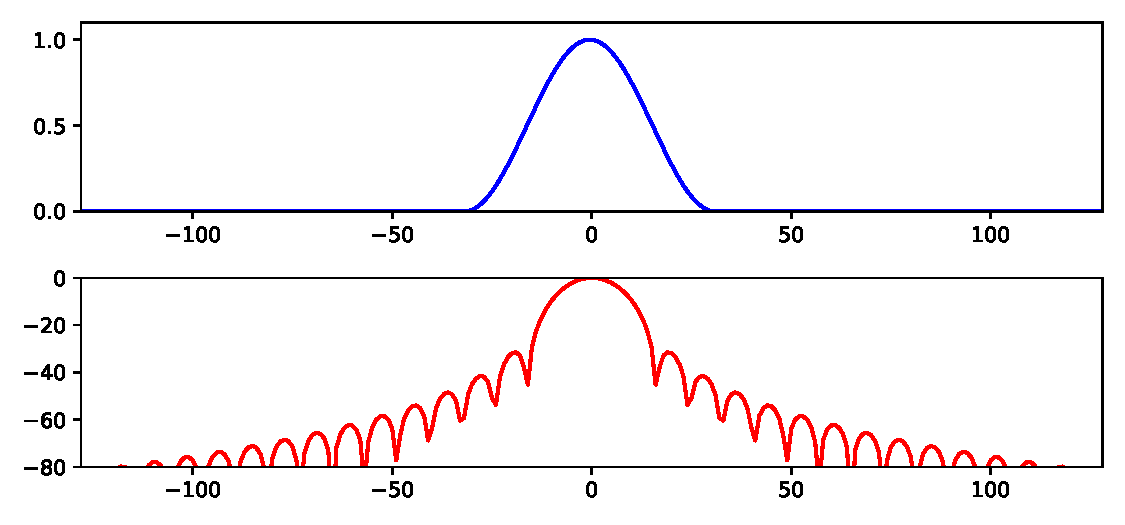
\includegraphics[width=\textwidth]{../fig/window_hann.pdf}
  \caption{Hann window and its spectrum}
  \label{fig:window_hann}
\end{figure}

\begin{figure}[htbp]
  \centering
  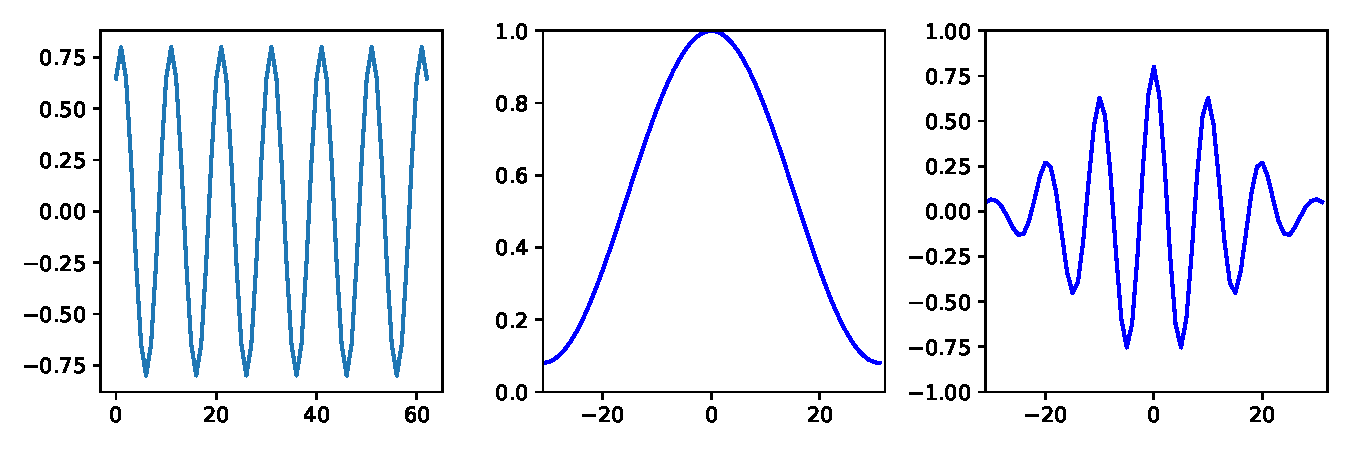
\includegraphics[width=\textwidth]{../fig/windowing_demo.pdf}
  \caption{An example of Hamming window (middle) applied to sinusoid signal (left); the resulted windowed signal (right) is multiplication of both.}
  \label{fig:windowing_demo}

\end{figure}
The length of a window is usually equal to the length of frame: one window per
frame. If the length of a window is smaller than a frame, each frame will be
windowed with window length and padded with zeros to match length of frame. It
costs more computation. In speech emotion recognition, short window is used to
capture short dynamics context while longer window is used to capture mid and
longer dynamics. A common approach used short window to extract acoustic
features in short-term time while long-term dynamics are modeled by statistical 
functions. Figure \ref{fig:frame-processing} shows frame-based processing of an
acoustic signal (speech) which windows short-term signals using Hamming window.

\begin{figure}[htbp]
  \centering
  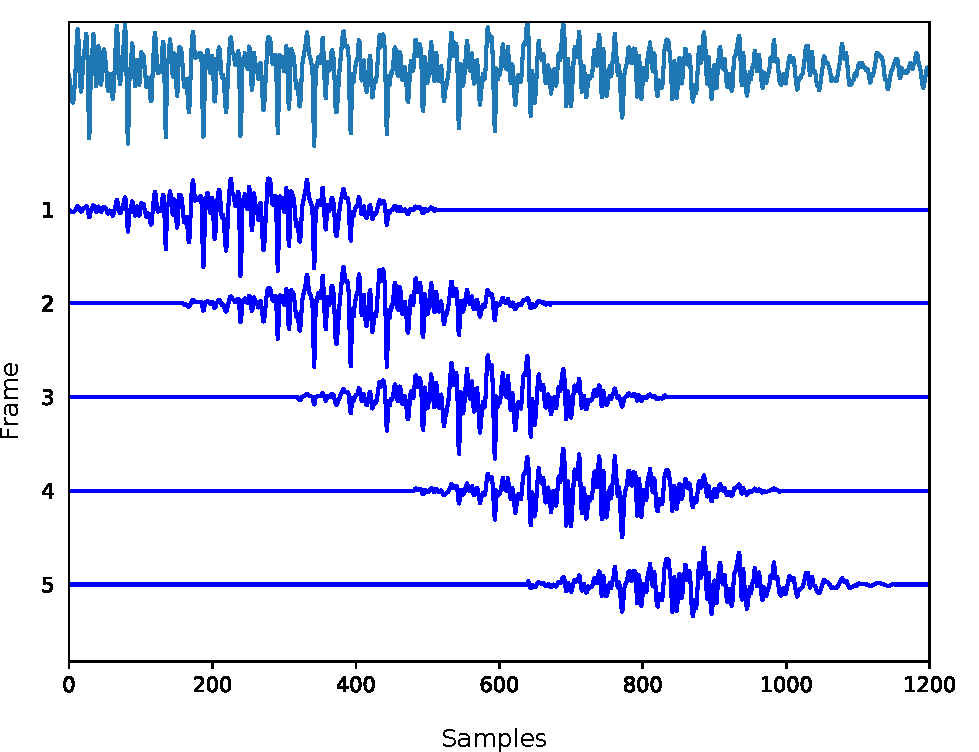
\includegraphics[width=\textwidth]{../fig/framing.pdf}  
  \caption{Frame-based processing for extracting low-level descriptors of an acoustic signal; the signal is an excerpt of IEMOCAP utterance with 400 samples frame length and 160 samples hop length; sampling frequency is 16 kHz.}
  \label{fig:frame-processing}
\end{figure}

% # LLD, MFCC, Why
The acoustic features extracted on each frame are known as local features or
low-level descriptor (LLD) \cite{Herrera1999}. The most common LLD for speech
processing is mel-frequency cepstral coefficients (MFCC). MFCC captures
different aspects of the spectral shape of a speech. The following steps
compute MFCC in sequences. First, FFT/DFT transformed time domain signal into
frequency domain signal (spectra). Second, mel frequency warping function
convert spectra in linear scale into mel scale. Although several functions have
been proposed, a common approach keeps linear scale for acoustic frequencies
below 1 kHz and converts to logarithmic scale for acoustic frequencies above 1
kHz. This conversion imitates human perceptual system. Third, convert a power
spectrogram (amplitude squared) to decibel (dB) units ($\log$). Finally, DCT
computes MFCC as amplitude cepstra.

% number of mfcc coefficients; number of frame; shape of MFCC
One of the important parameters in MFCC is the number of coefficients. A number
of 13 to 40 coefficients are common for speech processing. For
each frame 13 MFCCs are extracted. If there are 40 frames in an utterance, the
dimension of MFCC features will be (40, 13). Obviously, the number of frames
corresponds to the number of samples divided by hop length (in samples). 
If an utterance comprises 1 second (s) with 16000 Hz sampling rate, the
number of samples is 16000. Using 25 ms (400 samples) window/frame length and
10 ms (160 samples) hop length, the number of frames is $16000/160$, i.e.,
100 frames. Figure \ref{fig:mfcc_40} shows an MFCC spectrogram of an utterance
with 40 coefficients.

% mel-spectrogram and log mel-spectrogram
Recently, researchers found that mel-spectrogram, also called as (mel) filter
bank and mel frequency spectral coefficients (MFSC) for deep learning-based
automatic speech recognition (ASR) (e.g., \cite{Mohamed2014}). Given that deep
learning system is less susceptible with high correlated input, the DCT step in
previous MFCC calculation is not necessary since it is linear transformation.
DCT discards some information in speech signals which are highly non-linear
\cite{fayek2016}. Furthermore, a logarithmic version of mel-spectrogram, i.e.,
log mel-spectrogram, is preferable one since deep learning learns better in
this scale. The mel-spectrogram visualization as shown in Figure
\ref{fig:mfsc_128} support this argument in comparison with MFCC visualization.

% GeMAPS
Apart from the use of one type acoustic features for speech processing, some
researchers have proposed a set of acoustic features for speech emotion
recognition. Eyben et al. \cite{Eyben} proposed Geneva minimalistic parameter
set (GeMAPS) as standard acoustic features for affective voice research. The
proposed acoustic features are based on: (1) physiological changes in voice
production, (2) proven significance in previous studies, and (3) theoretical
significance. The proposed acoustic features comprises 23 LLDs as shown in
Table \ref{tab:gemaps_paa}. This acoustic feature set is extracted on
frame-processing basis with 25 ms frame length and 10 ms hop length.

% pyAudioanalysis
Giannakopulos \cite{Giannakopoulos2015} proposed pyAudioanalysis as an open
source Python library for audio signal analysis. The library supports a wide
range of audio analysis procedures such as feature extraction, classification,
supervised and unsupervised segmentation, and visualization. Different from
GeMAPS feature set, pyAudioanalysis targets a wide range of voice application
like audio event detection, speech emotion recognition, music segmentation, and
health application. The short-term feature set, which is extracted on
frame-processing basis, consists of 34 LLDs. These LLDs are shown in Table 
\ref{tab:gemaps_paa}.

\begin{table}[htpb]
  \centering
  \caption{Acoustic feature sets: GeMAPS \cite{Eyben} and pyAudioAnalysis \cite{Giannakopoulos2015}. The numbers in parentheses indicate the total numbers of features (LLDs).}
  \begin{tabular}{p{7.5cm} p{7cm}}
  \hline
  \hspace{2.5cm}GeMAPs (23) & \hspace{1.5cm}pyAudioAnalysis (34) \\
  \hline
intensity, alpha ratio, Hammarberg index, spectral slope 0-500 Hz, spectral
slope 500-1500 Hz, spectral flux, 4 MFCCs, F0, jitter, shimmer,
harmonics-to-noise ratio (HNR), harmonic difference H1-H2, harmonic difference
H1-A3, F1, F1 bandwidth, F1 amplitude, F2, F2 amplitude, F3, and F3 amplitude.
& zero crossing rate, energy, entropy of energy, spectral centroid, spectral
spread, spectral entropy, spectral flux, spectral roll-off, 13 MFCCs, 12 chroma
vectors, chroma deviation.\\
  \hline
  \end{tabular}
  \label{tab:gemaps_paa}
 \end{table}

% Result

% Summary LLD and Problem with frame-based processing: high-dimensions, needs
% zero padding

\section{SER using High-level Acoustic Features}

% \section{Evaluation Metric}
% \section{Experiment and Results on Region Analysis of Acoustic Features}
\section{Contribution of Silent Pause Features}
\section{Acoustic Features Aggregation}

% The content following two sections can be included in summary and previous
% sections
% \section{Effect of Different Acoustic Features}
% \section{Effect of Different Classifiers}
\section{Summary}



\renewcommand{\bibname}{References}
% \phantomsection
% \addcontentsline{toc}{chapter}{References}
\bibliographystyle{IEEEtran}
\bibliography{ref_s3}



% \strut
% \vspace{20pt}

\renewcommand{\nomname}{PUBLICATIONS}
\markboth{\nomname}{\nomname}
% \noindent{\LARGE\bf Publications}


% \vspace{20pt}
\addcontentsline{toc}{chapter}{Publications}

\begin{publication}
\item[] \hspace{-1cm}{\LARGE\bf Journals} \\ 

\item 
B. T. Atmaja and M. Akagi, ``Dimensional speech emotion recognition from speech
features and word embeddings by using multitask learning," APSIPA Trans. Signal
Inf. Process., Vol. 9, No. May, p. e17, May 2020.

\item
R. Elbarougy, B.T. Atmaja and M. Akagi, ``Continuous Audiovisual Emotion
Recognition Using Feature Selection and LSTM,'' Journal of Signal Processing,
Vol. 24, No. 6, November 2020. 

\item
B.T. Atmaja and M. Akagi, ``Two-stage dimensional emotion recognition by fusing
predictions of acoustic and text networks using SVM,'' Speech Communication,
vol 126, February 2021, pp 9-21.
\verb|doi:10.1016/j.specom.2020.11.003|. 

\item 
B.T. Atmaja and M. Akagi, ``Speech emotion recognition: From unimodal acoustic
analysis to bimodal acoustic-linguistic fusion,'' submitted to IEEE MultiMedia.
\\

\item[] \hspace{-1cm}{\LARGE\bf International Conferences} \\ 

\item 
B.T. Atmaja, K. Shirai, and M. Akagi, ``Deep Learning-based Categorical and
Dimensional Emotion Recognition for Written and Spoken Text,''
\textit{International Seminar on Science and Technology}, Surabaya, 2019.

\item 
B. T. Atmaja, K. Shirai, and M. Akagi, ``Speech Emotion Recognition Using
Speech Feature and Word Embedding," in 2019 Asia-Pacific Signal and Information
Processing Association Annual Summit and Conference (APSIPA ASC), 2019, pp.
519--523.

\item
B. T. Atmaja and M. Akagi, ``Speech Emotion Recognition Based on Speech Segment
Using LSTM with Attention Model," in 2019 IEEE International Conference on
Signals and Systems (ICSigSys), 2019, pp. 40--44.

\item
B. T. Atmaja and M. Akagi, ``Multitask Learning and Multistage Fusion for Dimensional Audiovisual Emotion Recognition," in ICASSP 2020 - 2020 IEEE International Conference on Acoustics, Speech and Signal Processing (ICASSP), 2020, pp. 4482--4486.

\item
B. T. Atmaja and M. Akagi, ``The Effect of Silence Feature in Dimensional
Speech Emotion Recognition," in 10th International Conference on Speech Prosody
2020, 2020, May, pp. 26--30.

\item
B.T. Atmaja and M. Akagi, ``Improving Valence Prediction in
Dimensional Speech Emotion Recognition Using Linguistic Information, " in 2020
23nd Conference of the Oriental COCOSDA International Committee for the
Co-ordination and Standardisation of Speech Databases and Assessment Techniques
(O-COCOSDA), pp. 166-171. IEEE, 2020. [\textbf{Awarded as best student paper}]

\item
B.T. Atmaja and M. Akagi, ``On The Differences Between Song and Speech Emotion
Recognition: Effect of Feature Sets, Feature Types, and Classifiers'', TENCON
2020 - 2020 IEEE Region 10 Conference (TENCON), Osaka, Japan, 2020.

\item
B.T. Atmaja, Y. Hamada  and M. Akagi, ``Predicting Valence and Arousal by Aggregating Acoustic Features for Acoustic-Linguistic Information Fusion''
TENCON 2020 - 2020 IEEE Region 10 Conference (TENCON), Osaka, Japan, 2020. 

\item 
B.T. Atmaja and M. Akagi, ``Deep Multilayer Perceptrons for Dimensional Speech
Emotion Recognition,'' in 2020 Asia-Pacific Signal and Information Processing
Association Annual Summit and Conference (APSIPA ASC), Auckland, New Zealand,
2020.

\item 
B.T. Atmaja and M. Akagi, ``Evaluation of Error and Correlation-based Loss
Functions For Multitask Learning Dimensional Speech Emotion Recognition,''
International Conference on Acoustic and Vibration, Bali, Indonesia, 2020.
[\textbf{Awarded as best student paper and presentation}]\\

\item[] \hspace{-1cm}{\LARGE\bf Domestic Conferences} \\ 
\item 
R. Elbarougy, B.T. Atmaja, and M. Akagi, ``Continuous Tracking of Emotional
State from Speech Based on Emotion Unit,''\textit{In Proceeding ASJ Autumn
Meeting}, 2018.

\item
B.T. Atmaja, A.N.F. Fandy, D. Arifianto, and M. Akagi, ``Speech recognition on
Indonesian language by using time delay neural network,'' \textit{In Proceeding
ASJ Spring Meeting}, 2019, pp. 1291--1294.

\item
B.T. Atmaja, R. Elbarougy, and M. Akagi, ``RNN-based dimensional speech emotion
recognition,'' \textit{In Proceeding ASJ Autumn Meeting}, 2019, pp. 743--744.

\item
B.T. Atmaja and M. Akagi, ``Dimensional Speech Emotion Recognition from
Acoustic and Text Features Using Multitask Learning,'' \textit{In Proceeding
ASJ Spring Meeting}, 2020, pp. 1003--1004.

\end{publication}


\end{document}
